% Options for packages loaded elsewhere
\PassOptionsToPackage{unicode}{hyperref}
\PassOptionsToPackage{hyphens}{url}
\PassOptionsToPackage{dvipsnames,svgnames,x11names}{xcolor}
%
\documentclass[
  letterpaper,
  DIV=11,
  numbers=noendperiod]{scrreprt}

\usepackage{amsmath,amssymb}
\usepackage{lmodern}
\usepackage{iftex}
\ifPDFTeX
  \usepackage[T1]{fontenc}
  \usepackage[utf8]{inputenc}
  \usepackage{textcomp} % provide euro and other symbols
\else % if luatex or xetex
  \usepackage{unicode-math}
  \defaultfontfeatures{Scale=MatchLowercase}
  \defaultfontfeatures[\rmfamily]{Ligatures=TeX,Scale=1}
\fi
% Use upquote if available, for straight quotes in verbatim environments
\IfFileExists{upquote.sty}{\usepackage{upquote}}{}
\IfFileExists{microtype.sty}{% use microtype if available
  \usepackage[]{microtype}
  \UseMicrotypeSet[protrusion]{basicmath} % disable protrusion for tt fonts
}{}
\makeatletter
\@ifundefined{KOMAClassName}{% if non-KOMA class
  \IfFileExists{parskip.sty}{%
    \usepackage{parskip}
  }{% else
    \setlength{\parindent}{0pt}
    \setlength{\parskip}{6pt plus 2pt minus 1pt}}
}{% if KOMA class
  \KOMAoptions{parskip=half}}
\makeatother
\usepackage{xcolor}
\setlength{\emergencystretch}{3em} % prevent overfull lines
\setcounter{secnumdepth}{5}
% Make \paragraph and \subparagraph free-standing
\ifx\paragraph\undefined\else
  \let\oldparagraph\paragraph
  \renewcommand{\paragraph}[1]{\oldparagraph{#1}\mbox{}}
\fi
\ifx\subparagraph\undefined\else
  \let\oldsubparagraph\subparagraph
  \renewcommand{\subparagraph}[1]{\oldsubparagraph{#1}\mbox{}}
\fi

\usepackage{color}
\usepackage{fancyvrb}
\newcommand{\VerbBar}{|}
\newcommand{\VERB}{\Verb[commandchars=\\\{\}]}
\DefineVerbatimEnvironment{Highlighting}{Verbatim}{commandchars=\\\{\}}
% Add ',fontsize=\small' for more characters per line
\usepackage{framed}
\definecolor{shadecolor}{RGB}{241,243,245}
\newenvironment{Shaded}{\begin{snugshade}}{\end{snugshade}}
\newcommand{\AlertTok}[1]{\textcolor[rgb]{0.68,0.00,0.00}{#1}}
\newcommand{\AnnotationTok}[1]{\textcolor[rgb]{0.37,0.37,0.37}{#1}}
\newcommand{\AttributeTok}[1]{\textcolor[rgb]{0.40,0.45,0.13}{#1}}
\newcommand{\BaseNTok}[1]{\textcolor[rgb]{0.68,0.00,0.00}{#1}}
\newcommand{\BuiltInTok}[1]{\textcolor[rgb]{0.00,0.23,0.31}{#1}}
\newcommand{\CharTok}[1]{\textcolor[rgb]{0.13,0.47,0.30}{#1}}
\newcommand{\CommentTok}[1]{\textcolor[rgb]{0.37,0.37,0.37}{#1}}
\newcommand{\CommentVarTok}[1]{\textcolor[rgb]{0.37,0.37,0.37}{\textit{#1}}}
\newcommand{\ConstantTok}[1]{\textcolor[rgb]{0.56,0.35,0.01}{#1}}
\newcommand{\ControlFlowTok}[1]{\textcolor[rgb]{0.00,0.23,0.31}{#1}}
\newcommand{\DataTypeTok}[1]{\textcolor[rgb]{0.68,0.00,0.00}{#1}}
\newcommand{\DecValTok}[1]{\textcolor[rgb]{0.68,0.00,0.00}{#1}}
\newcommand{\DocumentationTok}[1]{\textcolor[rgb]{0.37,0.37,0.37}{\textit{#1}}}
\newcommand{\ErrorTok}[1]{\textcolor[rgb]{0.68,0.00,0.00}{#1}}
\newcommand{\ExtensionTok}[1]{\textcolor[rgb]{0.00,0.23,0.31}{#1}}
\newcommand{\FloatTok}[1]{\textcolor[rgb]{0.68,0.00,0.00}{#1}}
\newcommand{\FunctionTok}[1]{\textcolor[rgb]{0.28,0.35,0.67}{#1}}
\newcommand{\ImportTok}[1]{\textcolor[rgb]{0.00,0.46,0.62}{#1}}
\newcommand{\InformationTok}[1]{\textcolor[rgb]{0.37,0.37,0.37}{#1}}
\newcommand{\KeywordTok}[1]{\textcolor[rgb]{0.00,0.23,0.31}{#1}}
\newcommand{\NormalTok}[1]{\textcolor[rgb]{0.00,0.23,0.31}{#1}}
\newcommand{\OperatorTok}[1]{\textcolor[rgb]{0.37,0.37,0.37}{#1}}
\newcommand{\OtherTok}[1]{\textcolor[rgb]{0.00,0.23,0.31}{#1}}
\newcommand{\PreprocessorTok}[1]{\textcolor[rgb]{0.68,0.00,0.00}{#1}}
\newcommand{\RegionMarkerTok}[1]{\textcolor[rgb]{0.00,0.23,0.31}{#1}}
\newcommand{\SpecialCharTok}[1]{\textcolor[rgb]{0.37,0.37,0.37}{#1}}
\newcommand{\SpecialStringTok}[1]{\textcolor[rgb]{0.13,0.47,0.30}{#1}}
\newcommand{\StringTok}[1]{\textcolor[rgb]{0.13,0.47,0.30}{#1}}
\newcommand{\VariableTok}[1]{\textcolor[rgb]{0.07,0.07,0.07}{#1}}
\newcommand{\VerbatimStringTok}[1]{\textcolor[rgb]{0.13,0.47,0.30}{#1}}
\newcommand{\WarningTok}[1]{\textcolor[rgb]{0.37,0.37,0.37}{\textit{#1}}}

\providecommand{\tightlist}{%
  \setlength{\itemsep}{0pt}\setlength{\parskip}{0pt}}\usepackage{longtable,booktabs,array}
\usepackage{calc} % for calculating minipage widths
% Correct order of tables after \paragraph or \subparagraph
\usepackage{etoolbox}
\makeatletter
\patchcmd\longtable{\par}{\if@noskipsec\mbox{}\fi\par}{}{}
\makeatother
% Allow footnotes in longtable head/foot
\IfFileExists{footnotehyper.sty}{\usepackage{footnotehyper}}{\usepackage{footnote}}
\makesavenoteenv{longtable}
\usepackage{graphicx}
\makeatletter
\def\maxwidth{\ifdim\Gin@nat@width>\linewidth\linewidth\else\Gin@nat@width\fi}
\def\maxheight{\ifdim\Gin@nat@height>\textheight\textheight\else\Gin@nat@height\fi}
\makeatother
% Scale images if necessary, so that they will not overflow the page
% margins by default, and it is still possible to overwrite the defaults
% using explicit options in \includegraphics[width, height, ...]{}
\setkeys{Gin}{width=\maxwidth,height=\maxheight,keepaspectratio}
% Set default figure placement to htbp
\makeatletter
\def\fps@figure{htbp}
\makeatother

\KOMAoption{captions}{tableheading}
\makeatletter
\@ifpackageloaded{tcolorbox}{}{\usepackage[many]{tcolorbox}}
\@ifpackageloaded{fontawesome5}{}{\usepackage{fontawesome5}}
\definecolor{quarto-callout-color}{HTML}{909090}
\definecolor{quarto-callout-note-color}{HTML}{0758E5}
\definecolor{quarto-callout-important-color}{HTML}{CC1914}
\definecolor{quarto-callout-warning-color}{HTML}{EB9113}
\definecolor{quarto-callout-tip-color}{HTML}{00A047}
\definecolor{quarto-callout-caution-color}{HTML}{FC5300}
\definecolor{quarto-callout-color-frame}{HTML}{acacac}
\definecolor{quarto-callout-note-color-frame}{HTML}{4582ec}
\definecolor{quarto-callout-important-color-frame}{HTML}{d9534f}
\definecolor{quarto-callout-warning-color-frame}{HTML}{f0ad4e}
\definecolor{quarto-callout-tip-color-frame}{HTML}{02b875}
\definecolor{quarto-callout-caution-color-frame}{HTML}{fd7e14}
\makeatother
\makeatletter
\makeatother
\makeatletter
\@ifpackageloaded{bookmark}{}{\usepackage{bookmark}}
\makeatother
\makeatletter
\@ifpackageloaded{caption}{}{\usepackage{caption}}
\AtBeginDocument{%
\ifdefined\contentsname
  \renewcommand*\contentsname{Table of contents}
\else
  \newcommand\contentsname{Table of contents}
\fi
\ifdefined\listfigurename
  \renewcommand*\listfigurename{List of Figures}
\else
  \newcommand\listfigurename{List of Figures}
\fi
\ifdefined\listtablename
  \renewcommand*\listtablename{List of Tables}
\else
  \newcommand\listtablename{List of Tables}
\fi
\ifdefined\figurename
  \renewcommand*\figurename{Figure}
\else
  \newcommand\figurename{Figure}
\fi
\ifdefined\tablename
  \renewcommand*\tablename{Table}
\else
  \newcommand\tablename{Table}
\fi
}
\@ifpackageloaded{float}{}{\usepackage{float}}
\floatstyle{ruled}
\@ifundefined{c@chapter}{\newfloat{codelisting}{h}{lop}}{\newfloat{codelisting}{h}{lop}[chapter]}
\floatname{codelisting}{Listing}
\newcommand*\listoflistings{\listof{codelisting}{List of Listings}}
\makeatother
\makeatletter
\@ifpackageloaded{caption}{}{\usepackage{caption}}
\@ifpackageloaded{subcaption}{}{\usepackage{subcaption}}
\makeatother
\makeatletter
\@ifpackageloaded{tcolorbox}{}{\usepackage[many]{tcolorbox}}
\makeatother
\makeatletter
\@ifundefined{shadecolor}{\definecolor{shadecolor}{rgb}{.97, .97, .97}}
\makeatother
\makeatletter
\makeatother
\ifLuaTeX
  \usepackage{selnolig}  % disable illegal ligatures
\fi
\IfFileExists{bookmark.sty}{\usepackage{bookmark}}{\usepackage{hyperref}}
\IfFileExists{xurl.sty}{\usepackage{xurl}}{} % add URL line breaks if available
\urlstyle{same} % disable monospaced font for URLs
\hypersetup{
  pdftitle={Principles and Techniques of Data Science},
  pdfauthor={Kanu Grover; Bella Crouch},
  colorlinks=true,
  linkcolor={blue},
  filecolor={Maroon},
  citecolor={Blue},
  urlcolor={Blue},
  pdfcreator={LaTeX via pandoc}}

\title{Principles and Techniques of Data Science}
\usepackage{etoolbox}
\makeatletter
\providecommand{\subtitle}[1]{% add subtitle to \maketitle
  \apptocmd{\@title}{\par {\large #1 \par}}{}{}
}
\makeatother
\subtitle{Data 100}
\author{Kanu Grover \and Bella Crouch}
\date{}

\begin{document}
\maketitle
\ifdefined\Shaded\renewenvironment{Shaded}{\begin{tcolorbox}[frame hidden, interior hidden, boxrule=0pt, borderline west={3pt}{0pt}{shadecolor}, enhanced, sharp corners, breakable]}{\end{tcolorbox}}\fi

\renewcommand*\contentsname{Table of contents}
{
\hypersetup{linkcolor=}
\setcounter{tocdepth}{2}
\tableofcontents
}
\bookmarksetup{startatroot}

\hypertarget{welcome}{%
\chapter*{Welcome}\label{welcome}}
\addcontentsline{toc}{chapter}{Welcome}

\markboth{Welcome}{Welcome}

This text was originally developed for the Spring 2023 Edition of the UC
Berkeley course Data 100: Principles and Techniques of Data Science.

\bookmarksetup{startatroot}

\hypertarget{introduction}{%
\chapter{Introduction}\label{introduction}}

\begin{tcolorbox}[enhanced jigsaw, toprule=.15mm, rightrule=.15mm, colback=white, opacitybacktitle=0.6, toptitle=1mm, bottomrule=.15mm, titlerule=0mm, colbacktitle=quarto-callout-note-color!10!white, opacityback=0, leftrule=.75mm, arc=.35mm, bottomtitle=1mm, title=\textcolor{quarto-callout-note-color}{\faInfo}\hspace{0.5em}{Note}, left=2mm, breakable, coltitle=black, colframe=quarto-callout-note-color-frame]

\begin{itemize}
\tightlist
\item
  Understand the stages of the data science lifecycle.
\end{itemize}

\end{tcolorbox}

Data science is an interdisciplinary field with a variety of
applications. The field is rapidly evolving; many of the key technical
underpinnings in modern-day data science have been popularized during
the early 21\textsuperscript{st} century.

A true mastery of data science requires a deep theoretical understanding
and strong grasp of domain expertise. This course will help you build on
the former -- specifically, the foundation of your technical knowledge.
To do so, we've organized concepts in Data 100 around the \textbf{data
science lifecycle}: an iterative process that encompasses the various
statistical and computational building blocks of data science.

\hypertarget{data-science-lifecycle}{%
\section{Data Science Lifecycle}\label{data-science-lifecycle}}

The data science lifecycle is a high-level overview of the data science
workflow. It is a cycle of stages that a data scientist must explore as
they conduct a thorough analysis of a data-driven problem.

There are many variations of the key ideas present in the data science
lifecycle. In Data 100, we visualize the stages of the lifecycle using a
flow diagram. Notice how there are two entry points.

\hypertarget{ask-a-question}{%
\subsection{Ask a Question}\label{ask-a-question}}

Whether by curiosity or necessity, data scientists will constantly ask
questions. For example, in the business world, data scientists may be
interested in predicting the profit generated by a certain investment.
In the field of medicine, they may ask whether some patients are more
likely than others to benefit from a treatment.

Posing questions are one of the primary ways by which the data science
lifecycle beings. It helps to fully define the question. Here are some
things you should ask yourself before framing a question.

\begin{itemize}
\tightlist
\item
  What do we want to know?

  \begin{itemize}
  \tightlist
  \item
    A question that is too ambiguous may lead to confusion.
  \end{itemize}
\item
  What problems are we trying to solve?

  \begin{itemize}
  \tightlist
  \item
    The goal of asking a question should be clear in order to justify
    your efforts to stakeholders.
  \end{itemize}
\item
  What are the hypotheses we want to test?

  \begin{itemize}
  \tightlist
  \item
    This gives a clear perspective from which to analyze final results.
  \end{itemize}
\item
  What are the metrics for our success?

  \begin{itemize}
  \tightlist
  \item
    This gives a clear point to know when to finish the project.
  \end{itemize}
\end{itemize}

\hypertarget{obtain-data}{%
\subsection{Obtain Data}\label{obtain-data}}

The second entry point to the lifecycle is by obtaining data. A careful
analysis of any problem requires the use of data. Data may be readily
available to us, or we may have to embark on a process to collect it.
When doing so, its crucial to ask the following:

\begin{itemize}
\tightlist
\item
  What data do we have and what data do we need?

  \begin{itemize}
  \tightlist
  \item
    Define the units of the data (people, cities, points in time, etc.)
    and what features to measure.
  \end{itemize}
\item
  How will we sample more data?

  \begin{itemize}
  \tightlist
  \item
    Scrape the web, collect manually, etc.
  \end{itemize}
\item
  Is our data representative of the population we want to study?

  \begin{itemize}
  \tightlist
  \item
    If our data is not representative of our population of interest,
    then we can come to incorrect conclusions.
  \end{itemize}
\end{itemize}

Key procedures: \emph{data acquisition}, \emph{data cleaning}

\hypertarget{understand-the-data}{%
\subsection{Understand the Data}\label{understand-the-data}}

Raw data itself is not inherently useful. It's impossible to discern all
the patterns and relationships between variables without carefully
investigating them. Therefore, translating pure data to actionable
insights is a key job of a data scientist. For example, we may choose to
ask:

\begin{itemize}
\tightlist
\item
  How is our data organized and what does it contain?

  \begin{itemize}
  \tightlist
  \item
    Knowing what the data says about the world helps us better
    understand the world.
  \end{itemize}
\item
  Do we have relevant data?

  \begin{itemize}
  \tightlist
  \item
    If the data we have collected is not useful to the question at hand,
    then we must collected more data.
  \end{itemize}
\item
  What are the biases, anomalies, or other issues with the data?

  \begin{itemize}
  \tightlist
  \item
    These can lead to many false conclusions if ignored, so data
    scientists must always be aware of these issues.
  \end{itemize}
\item
  How do we transform the data to enable effective analysis?

  \begin{itemize}
  \tightlist
  \item
    Data is not always easy to interpret at first glance, so a data
    scientist should reveal these hidden insights.
  \end{itemize}
\end{itemize}

Key procedures: \emph{exploratory data analysis}, \emph{data
visualization}.

\hypertarget{understand-the-world}{%
\subsection{Understand the World}\label{understand-the-world}}

After observing the patterns in our data, we turn to answering our
problem. This may require that we predict a quantity (machine learning),
or measure the effect of some treatment (inference).

From here, we may choose to report our results, or possibly conduct more
analysis. We may not be satisfied by our findings, or our initial
exploration may have brought up new questions that require a new
perspective.

\begin{itemize}
\tightlist
\item
  What does the data say about the world?

  \begin{itemize}
  \tightlist
  \item
    Given our models, the data will lead us to certain conclusions about
    the real world.\\
  \end{itemize}
\item
  Does it answer our questions or accurately solve the problem?

  \begin{itemize}
  \tightlist
  \item
    If our model and data can not accomplish our goals, then we must
    reform our question, model, or both.\\
  \end{itemize}
\item
  How robust are our conclusions and can we trust the predictions?

  \begin{itemize}
  \tightlist
  \item
    Inaccurate models can lead to untrue conclusions.
  \end{itemize}
\end{itemize}

Key procedures: \emph{model creation}, \emph{prediction},
\emph{inference}.

\hypertarget{conclusion}{%
\section{Conclusion}\label{conclusion}}

The data science lifecycle is meant to be a set of general guidelines
rather than a hard list of requirements. In our journey exploring the
lifecycle, we'll cover both the underlying theory and technologies used
in data science, and we hope you'll build an appreciation for the field.

With that, let's begin by introducing one of the most important tools in
data analysis: \texttt{pandas}.

\bookmarksetup{startatroot}

\hypertarget{pandas-i}{%
\chapter{Pandas I}\label{pandas-i}}

\begin{tcolorbox}[enhanced jigsaw, toprule=.15mm, rightrule=.15mm, colback=white, opacitybacktitle=0.6, toptitle=1mm, bottomrule=.15mm, titlerule=0mm, colbacktitle=quarto-callout-note-color!10!white, opacityback=0, leftrule=.75mm, arc=.35mm, bottomtitle=1mm, title=\textcolor{quarto-callout-note-color}{\faInfo}\hspace{0.5em}{Note}, left=2mm, breakable, coltitle=black, colframe=quarto-callout-note-color-frame]

\begin{itemize}
\tightlist
\item
  Build familiarity with basic \texttt{pandas} syntax
\item
  Learn the methods of selecting and filtering data from a DataFrame.
\item
  Understand the differences between DataFrames and Series
\end{itemize}

\end{tcolorbox}

Data scientists work with data stored in a variety of formats. The
primary focus of this class is in understanding tabular data - one of
the most widely used formats in data science. This note introduces
DataFrames, which are among the most popular representations of tabular
data. We'll also introduce \texttt{pandas}, the standard Python package
for manipulating data in DataFrames.

\hypertarget{dataframes}{%
\section{DataFrames}\label{dataframes}}

In Data 8, you encountered the \texttt{Table} class of the
\texttt{datascience} library. In Data 100, we'll be using the
\texttt{DataFrame} class of the \texttt{pandas} library.

Here is an example of a DataFrame containing election data.

\begin{Shaded}
\begin{Highlighting}[]
\ImportTok{import}\NormalTok{ pandas }\ImportTok{as}\NormalTok{ pd}

\NormalTok{elections }\OperatorTok{=}\NormalTok{ pd.read\_csv(}\StringTok{"data/elections.csv"}\NormalTok{)}
\NormalTok{elections}
\end{Highlighting}
\end{Shaded}

\begin{tabular}{lrllrlr}
\toprule
{} &  Year &               Candidate &                  Party &  Popular vote & Result &          \% \\
\midrule
0   &  1824 &          Andrew Jackson &  Democratic-Republican &        151271 &   loss &  57.210122 \\
1   &  1824 &       John Quincy Adams &  Democratic-Republican &        113142 &    win &  42.789878 \\
2   &  1828 &          Andrew Jackson &             Democratic &        642806 &    win &  56.203927 \\
3   &  1828 &       John Quincy Adams &    National Republican &        500897 &   loss &  43.796073 \\
4   &  1832 &          Andrew Jackson &             Democratic &        702735 &    win &  54.574789 \\
5   &  1832 &              Henry Clay &    National Republican &        484205 &   loss &  37.603628 \\
6   &  1832 &            William Wirt &           Anti-Masonic &        100715 &   loss &   7.821583 \\
7   &  1836 &       Hugh Lawson White &                   Whig &        146109 &   loss &  10.005985 \\
8   &  1836 &        Martin Van Buren &             Democratic &        763291 &    win &  52.272472 \\
9   &  1836 &  William Henry Harrison &                   Whig &        550816 &   loss &  37.721543 \\
10  &  1840 &        Martin Van Buren &             Democratic &       1128854 &   loss &  46.948787 \\
11  &  1840 &  William Henry Harrison &                   Whig &       1275583 &    win &  53.051213 \\
12  &  1844 &              Henry Clay &                   Whig &       1300004 &   loss &  49.250523 \\
13  &  1844 &              James Polk &             Democratic &       1339570 &    win &  50.749477 \\
14  &  1848 &              Lewis Cass &             Democratic &       1223460 &   loss &  42.552229 \\
15  &  1848 &        Martin Van Buren &              Free Soil &        291501 &   loss &  10.138474 \\
16  &  1848 &          Zachary Taylor &                   Whig &       1360235 &    win &  47.309296 \\
17  &  1852 &         Franklin Pierce &             Democratic &       1605943 &    win &  51.013168 \\
18  &  1852 &            John P. Hale &              Free Soil &        155210 &   loss &   4.930283 \\
19  &  1852 &          Winfield Scott &                   Whig &       1386942 &   loss &  44.056548 \\
20  &  1856 &          James Buchanan &             Democratic &       1835140 &    win &  45.306080 \\
21  &  1856 &         John C. Frémont &             Republican &       1342345 &   loss &  33.139919 \\
22  &  1856 &        Millard Fillmore &               American &        873053 &   loss &  21.554001 \\
23  &  1860 &         Abraham Lincoln &             Republican &       1855993 &    win &  39.699408 \\
24  &  1860 &               John Bell &   Constitutional Union &        590901 &   loss &  12.639283 \\
25  &  1860 &    John C. Breckinridge &    Southern Democratic &        848019 &   loss &  18.138998 \\
26  &  1860 &      Stephen A. Douglas &    Northern Democratic &       1380202 &   loss &  29.522311 \\
27  &  1864 &         Abraham Lincoln &         National Union &       2211317 &    win &  54.951512 \\
28  &  1864 &     George B. McClellan &             Democratic &       1812807 &   loss &  45.048488 \\
29  &  1868 &         Horatio Seymour &             Democratic &       2708744 &   loss &  47.334695 \\
30  &  1868 &           Ulysses Grant &             Republican &       3013790 &    win &  52.665305 \\
31  &  1872 &          Horace Greeley &     Liberal Republican &       2834761 &   loss &  44.071406 \\
32  &  1872 &           Ulysses Grant &             Republican &       3597439 &    win &  55.928594 \\
33  &  1876 &        Rutherford Hayes &             Republican &       4034142 &    win &  48.471624 \\
34  &  1876 &        Samuel J. Tilden &             Democratic &       4288546 &   loss &  51.528376 \\
35  &  1880 &         James B. Weaver &              Greenback &        308649 &   loss &   3.352344 \\
36  &  1880 &          James Garfield &             Republican &       4453337 &    win &  48.369234 \\
37  &  1880 &  Winfield Scott Hancock &             Democratic &       4444976 &   loss &  48.278422 \\
38  &  1884 &         Benjamin Butler &          Anti-Monopoly &        134294 &   loss &   1.335838 \\
39  &  1884 &        Grover Cleveland &             Democratic &       4914482 &    win &  48.884933 \\
40  &  1884 &         James G. Blaine &             Republican &       4856905 &   loss &  48.312208 \\
41  &  1884 &           John St. John &            Prohibition &        147482 &   loss &   1.467021 \\
42  &  1888 &          Alson Streeter &            Union Labor &        146602 &   loss &   1.288861 \\
43  &  1888 &       Benjamin Harrison &             Republican &       5443633 &    win &  47.858041 \\
44  &  1888 &         Clinton B. Fisk &            Prohibition &        249819 &   loss &   2.196299 \\
45  &  1888 &        Grover Cleveland &             Democratic &       5534488 &   loss &  48.656799 \\
46  &  1892 &       Benjamin Harrison &             Republican &       5176108 &   loss &  42.984101 \\
47  &  1892 &        Grover Cleveland &             Democratic &       5553898 &    win &  46.121393 \\
48  &  1892 &         James B. Weaver &               Populist &       1041028 &   loss &   8.645038 \\
49  &  1892 &            John Bidwell &            Prohibition &        270879 &   loss &   2.249468 \\
50  &  1896 &          John M. Palmer &    National Democratic &        134645 &   loss &   0.969566 \\
51  &  1896 &         Joshua Levering &            Prohibition &        131312 &   loss &   0.945565 \\
52  &  1896 &  William Jennings Bryan &             Democratic &       6509052 &   loss &  46.871053 \\
53  &  1896 &        William McKinley &             Republican &       7112138 &    win &  51.213817 \\
54  &  1900 &         John G. Woolley &            Prohibition &        210864 &   loss &   1.526821 \\
55  &  1900 &  William Jennings Bryan &             Democratic &       6370932 &   loss &  46.130540 \\
56  &  1900 &        William McKinley &             Republican &       7228864 &    win &  52.342640 \\
57  &  1904 &         Alton B. Parker &             Democratic &       5083880 &   loss &  37.685116 \\
58  &  1904 &          Eugene V. Debs &              Socialist &        402810 &   loss &   2.985897 \\
59  &  1904 &        Silas C. Swallow &            Prohibition &        259102 &   loss &   1.920637 \\
60  &  1904 &      Theodore Roosevelt &             Republican &       7630557 &    win &  56.562787 \\
61  &  1904 &        Thomas E. Watson &               Populist &        114070 &   loss &   0.845563 \\
62  &  1908 &          Eugene V. Debs &              Socialist &        420852 &   loss &   2.850866 \\
63  &  1908 &        Eugene W. Chafin &            Prohibition &        254087 &   loss &   1.721194 \\
64  &  1908 &  William Jennings Bryan &             Democratic &       6408979 &   loss &  43.414640 \\
65  &  1908 &            William Taft &             Republican &       7678335 &    win &  52.013300 \\
66  &  1912 &          Eugene V. Debs &              Socialist &        901551 &   loss &   6.004354 \\
67  &  1912 &        Eugene W. Chafin &            Prohibition &        208156 &   loss &   1.386325 \\
68  &  1912 &      Theodore Roosevelt &            Progressive &       4122721 &   loss &  27.457433 \\
69  &  1912 &            William Taft &             Republican &       3486242 &   loss &  23.218466 \\
70  &  1912 &          Woodrow Wilson &             Democratic &       6296284 &    win &  41.933422 \\
71  &  1916 &         Allan L. Benson &              Socialist &        590524 &   loss &   3.194193 \\
72  &  1916 &    Charles Evans Hughes &             Republican &       8548728 &   loss &  46.240779 \\
73  &  1916 &             Frank Hanly &            Prohibition &        221302 &   loss &   1.197041 \\
74  &  1916 &          Woodrow Wilson &             Democratic &       9126868 &    win &  49.367987 \\
75  &  1920 &        Aaron S. Watkins &            Prohibition &        188787 &   loss &   0.708351 \\
76  &  1920 &          Eugene V. Debs &              Socialist &        913693 &   loss &   3.428282 \\
77  &  1920 &            James M. Cox &             Democratic &       9139661 &   loss &  34.293063 \\
78  &  1920 &   Parley P. Christensen &           Farmer–Labor &        265398 &   loss &   0.995804 \\
79  &  1920 &          Warren Harding &             Republican &      16144093 &    win &  60.574501 \\
80  &  1924 &         Calvin Coolidge &             Republican &      15723789 &    win &  54.329113 \\
81  &  1924 &           John W. Davis &             Democratic &       8386242 &   loss &  28.976291 \\
82  &  1924 &      Robert La Follette &            Progressive &       4831706 &   loss &  16.694596 \\
83  &  1928 &                Al Smith &             Democratic &      15015464 &   loss &  40.902853 \\
84  &  1928 &          Herbert Hoover &             Republican &      21427123 &    win &  58.368524 \\
85  &  1928 &           Norman Thomas &              Socialist &        267478 &   loss &   0.728623 \\
86  &  1932 &      Franklin Roosevelt &             Democratic &      22821277 &    win &  57.672125 \\
87  &  1932 &          Herbert Hoover &             Republican &      15761254 &   loss &  39.830594 \\
88  &  1932 &           Norman Thomas &              Socialist &        884885 &   loss &   2.236211 \\
89  &  1932 &       William Z. Foster &              Communist &        103307 &   loss &   0.261069 \\
90  &  1936 &              Alf Landon &             Republican &      16679543 &   loss &  36.648285 \\
91  &  1936 &      Franklin Roosevelt &             Democratic &      27752648 &    win &  60.978107 \\
92  &  1936 &           Norman Thomas &              Socialist &        187910 &   loss &   0.412876 \\
93  &  1936 &           William Lemke &                  Union &        892378 &   loss &   1.960733 \\
94  &  1940 &      Franklin Roosevelt &             Democratic &      27313945 &    win &  54.871202 \\
95  &  1940 &           Norman Thomas &              Socialist &        116599 &   loss &   0.234237 \\
96  &  1940 &         Wendell Willkie &             Republican &      22347744 &   loss &  44.894561 \\
97  &  1944 &      Franklin Roosevelt &             Democratic &      25612916 &    win &  53.773801 \\
98  &  1944 &         Thomas E. Dewey &             Republican &      22017929 &   loss &  46.226199 \\
99  &  1948 &        Claude A. Watson &            Prohibition &        103708 &   loss &   0.212747 \\
100 &  1948 &            Harry Truman &             Democratic &      24179347 &    win &  49.601536 \\
101 &  1948 &        Henry A. Wallace &            Progressive &       1157328 &   loss &   2.374144 \\
102 &  1948 &           Norman Thomas &              Socialist &        139569 &   loss &   0.286312 \\
103 &  1948 &          Strom Thurmond &              Dixiecrat &       1175930 &   loss &   2.412304 \\
104 &  1948 &         Thomas E. Dewey &             Republican &      21991292 &   loss &  45.112958 \\
105 &  1952 &         Adlai Stevenson &             Democratic &      27375090 &   loss &  44.446312 \\
106 &  1952 &       Dwight Eisenhower &             Republican &      34075529 &    win &  55.325173 \\
107 &  1952 &        Vincent Hallinan &            Progressive &        140746 &   loss &   0.228516 \\
108 &  1956 &         Adlai Stevenson &             Democratic &      26028028 &   loss &  42.174464 \\
109 &  1956 &       Dwight Eisenhower &             Republican &      35579180 &    win &  57.650654 \\
110 &  1956 &      T. Coleman Andrews &         States' Rights &        107929 &   loss &   0.174883 \\
111 &  1960 &            John Kennedy &             Democratic &      34220984 &    win &  50.082561 \\
112 &  1960 &           Richard Nixon &             Republican &      34108157 &   loss &  49.917439 \\
113 &  1964 &         Barry Goldwater &             Republican &      27175754 &   loss &  38.655297 \\
114 &  1964 &          Lyndon Johnson &             Democratic &      43127041 &    win &  61.344703 \\
115 &  1968 &          George Wallace &   American Independent &       9901118 &   loss &  13.571218 \\
116 &  1968 &         Hubert Humphrey &             Democratic &      31271839 &   loss &  42.863537 \\
117 &  1968 &           Richard Nixon &             Republican &      31783783 &    win &  43.565246 \\
118 &  1972 &         George McGovern &             Democratic &      29173222 &   loss &  37.670670 \\
119 &  1972 &         John G. Schmitz &   American Independent &       1100868 &   loss &   1.421524 \\
120 &  1972 &           Richard Nixon &             Republican &      47168710 &    win &  60.907806 \\
121 &  1976 &         Eugene McCarthy &            Independent &        740460 &   loss &   0.911649 \\
122 &  1976 &             Gerald Ford &             Republican &      39148634 &   loss &  48.199499 \\
123 &  1976 &            Jimmy Carter &             Democratic &      40831881 &    win &  50.271900 \\
124 &  1976 &           Lester Maddox &   American Independent &        170274 &   loss &   0.209640 \\
125 &  1976 &          Roger MacBride &            Libertarian &        172557 &   loss &   0.212451 \\
126 &  1976 &      Thomas J. Anderson &               American &        158271 &   loss &   0.194862 \\
127 &  1980 &          Barry Commoner &               Citizens &        233052 &   loss &   0.270182 \\
128 &  1980 &                Ed Clark &            Libertarian &        921128 &   loss &   1.067883 \\
129 &  1980 &            Jimmy Carter &             Democratic &      35480115 &   loss &  41.132848 \\
130 &  1980 &        John B. Anderson &            Independent &       5719850 &   loss &   6.631143 \\
131 &  1980 &           Ronald Reagan &             Republican &      43903230 &    win &  50.897944 \\
132 &  1984 &          David Bergland &            Libertarian &        228111 &   loss &   0.247245 \\
133 &  1984 &           Ronald Reagan &             Republican &      54455472 &    win &  59.023326 \\
134 &  1984 &          Walter Mondale &             Democratic &      37577352 &   loss &  40.729429 \\
135 &  1988 &       George H. W. Bush &             Republican &      48886597 &    win &  53.518845 \\
136 &  1988 &           Lenora Fulani &           New Alliance &        217221 &   loss &   0.237804 \\
137 &  1988 &         Michael Dukakis &             Democratic &      41809074 &   loss &  45.770691 \\
138 &  1988 &                Ron Paul &            Libertarian &        431750 &   loss &   0.472660 \\
139 &  1992 &            Andre Marrou &            Libertarian &        290087 &   loss &   0.278516 \\
140 &  1992 &            Bill Clinton &             Democratic &      44909806 &    win &  43.118485 \\
141 &  1992 &                Bo Gritz &               Populist &        106152 &   loss &   0.101918 \\
142 &  1992 &       George H. W. Bush &             Republican &      39104550 &   loss &  37.544784 \\
143 &  1992 &              Ross Perot &            Independent &      19743821 &   loss &  18.956298 \\
144 &  1996 &            Bill Clinton &             Democratic &      47400125 &    win &  49.296938 \\
145 &  1996 &                Bob Dole &             Republican &      39197469 &   loss &  40.766036 \\
146 &  1996 &            Harry Browne &            Libertarian &        485759 &   loss &   0.505198 \\
147 &  1996 &         Howard Phillips &              Taxpayers &        184656 &   loss &   0.192045 \\
148 &  1996 &            John Hagelin &            Natural Law &        113670 &   loss &   0.118219 \\
149 &  1996 &             Ralph Nader &                  Green &        685297 &   loss &   0.712721 \\
150 &  1996 &              Ross Perot &                 Reform &       8085294 &   loss &   8.408844 \\
151 &  2000 &                 Al Gore &             Democratic &      50999897 &   loss &  48.491813 \\
152 &  2000 &          George W. Bush &             Republican &      50456002 &    win &  47.974666 \\
153 &  2000 &            Harry Browne &            Libertarian &        384431 &   loss &   0.365525 \\
154 &  2000 &            Pat Buchanan &                 Reform &        448895 &   loss &   0.426819 \\
155 &  2000 &             Ralph Nader &                  Green &       2882955 &   loss &   2.741176 \\
156 &  2004 &              David Cobb &                  Green &        119859 &   loss &   0.098088 \\
157 &  2004 &          George W. Bush &             Republican &      62040610 &    win &  50.771824 \\
158 &  2004 &              John Kerry &             Democratic &      59028444 &   loss &  48.306775 \\
159 &  2004 &        Michael Badnarik &            Libertarian &        397265 &   loss &   0.325108 \\
160 &  2004 &        Michael Peroutka &           Constitution &        143630 &   loss &   0.117542 \\
161 &  2004 &             Ralph Nader &            Independent &        465151 &   loss &   0.380663 \\
162 &  2008 &            Barack Obama &             Democratic &      69498516 &    win &  53.023510 \\
163 &  2008 &                Bob Barr &            Libertarian &        523715 &   loss &   0.399565 \\
164 &  2008 &           Chuck Baldwin &           Constitution &        199750 &   loss &   0.152398 \\
165 &  2008 &        Cynthia McKinney &                  Green &        161797 &   loss &   0.123442 \\
166 &  2008 &             John McCain &             Republican &      59948323 &   loss &  45.737243 \\
167 &  2008 &             Ralph Nader &            Independent &        739034 &   loss &   0.563842 \\
168 &  2012 &            Barack Obama &             Democratic &      65915795 &    win &  51.258484 \\
169 &  2012 &            Gary Johnson &            Libertarian &       1275971 &   loss &   0.992241 \\
170 &  2012 &              Jill Stein &                  Green &        469627 &   loss &   0.365199 \\
171 &  2012 &             Mitt Romney &             Republican &      60933504 &   loss &  47.384076 \\
172 &  2016 &          Darrell Castle &           Constitution &        203091 &   loss &   0.149640 \\
173 &  2016 &            Donald Trump &             Republican &      62984828 &    win &  46.407862 \\
174 &  2016 &           Evan McMullin &            Independent &        732273 &   loss &   0.539546 \\
175 &  2016 &            Gary Johnson &            Libertarian &       4489235 &   loss &   3.307714 \\
176 &  2016 &         Hillary Clinton &             Democratic &      65853514 &   loss &  48.521539 \\
177 &  2016 &              Jill Stein &                  Green &       1457226 &   loss &   1.073699 \\
178 &  2020 &            Joseph Biden &             Democratic &      81268924 &    win &  51.311515 \\
179 &  2020 &            Donald Trump &             Republican &      74216154 &   loss &  46.858542 \\
180 &  2020 &            Jo Jorgensen &            Libertarian &       1865724 &   loss &   1.177979 \\
181 &  2020 &          Howard Hawkins &                  Green &        405035 &   loss &   0.255731 \\
\bottomrule
\end{tabular}

Let's dissect the code above.

\begin{enumerate}
\def\labelenumi{\arabic{enumi}.}
\item
  We first import the \texttt{pandas} library into our Python
  environment, using the alias \texttt{pd}.
   \texttt{import\ pandas\ as\ pd}
\item
  There are a number of ways to read data into a DataFrame. In Data 100,
  our data are typically stored in a CSV (comma-seperated values) file
  format. We can import a CSV file into a DataFrame by passing the data
  path as an argument to the following \texttt{pandas} function.
   \texttt{pd.read\_csv("elections.csv")}
\end{enumerate}

This code stores our DataFrame object into the \texttt{elections}
variable. Upon inspection, our \texttt{elections} DataFrame has 182 rows
and 6 columns. Each row represents a single record - in our example, a
presedential candidate from some particular year. Each column represents
a single attribute, or feature of the record.

The API (application programming interface) for the DataFrame class is
enormous. In the next section, we'll discuss several methods of the
DataFrame API that allow us to extract subsets of data.

\hypertarget{slicing-in-dataframes}{%
\section{Slicing in DataFrames}\label{slicing-in-dataframes}}

The most fundamental way to manipulate a DataFrame is to extract a
subset of rows and columns. This is called \textbf{slicing}. We will do
so with three primary methods of the DataFrame class:

\begin{enumerate}
\def\labelenumi{\arabic{enumi}.}
\tightlist
\item
  \texttt{.loc}
\item
  \texttt{.iloc}
\item
  \texttt{{[}{]}}
\end{enumerate}

\hypertarget{indexing-with-.loc}{%
\subsection{Indexing with .loc}\label{indexing-with-.loc}}

The \texttt{.loc} operator selects rows and columns in a DataFrame by
their row and column label(s), respectively. The \textbf{row label}
(commonly referred to as the \textbf{index}) is the bold text on the far
\emph{left} of a DataFrame, while the \textbf{column label} is the text
found at the \emph{top} of a DataFrame. By default, row labels in
\texttt{pandas} are the sequential list of integers beginning from 0.
The column labels in our \texttt{elections} DataFrame are the column
names themselves: \texttt{Year}, \texttt{Candidate}, \texttt{Party},
\texttt{Popular\ Vote}, \texttt{Result}, and \texttt{\%}.

\texttt{.loc} lets us grab data by specifying the appropriate row and
column label(s) where the data exists. The row labels are the first
argument to the \texttt{.loc} function; the column labels are the
second. For example, to select the the row labeled \texttt{0} and the
column labeled \texttt{Candidate} from our \texttt{elections} DataFrame
we can write:

\begin{Shaded}
\begin{Highlighting}[]
\NormalTok{elections.loc[}\DecValTok{0}\NormalTok{, }\StringTok{\textquotesingle{}Candidate\textquotesingle{}}\NormalTok{]}
\end{Highlighting}
\end{Shaded}

\begin{verbatim}
'Andrew Jackson'
\end{verbatim}

To select \emph{multiple} rows and columns, we can use Python slice
notation. We can select the first four rows and first four columns.

\begin{Shaded}
\begin{Highlighting}[]
\NormalTok{elections.loc[}\DecValTok{0}\NormalTok{:}\DecValTok{3}\NormalTok{, }\StringTok{\textquotesingle{}Year\textquotesingle{}}\NormalTok{:}\StringTok{\textquotesingle{}Popular vote\textquotesingle{}}\NormalTok{]}
\end{Highlighting}
\end{Shaded}

\begin{tabular}{lrllr}
\toprule
{} &  Year &          Candidate &                  Party &  Popular vote \\
\midrule
0 &  1824 &     Andrew Jackson &  Democratic-Republican &        151271 \\
1 &  1824 &  John Quincy Adams &  Democratic-Republican &        113142 \\
2 &  1828 &     Andrew Jackson &             Democratic &        642806 \\
3 &  1828 &  John Quincy Adams &    National Republican &        500897 \\
\bottomrule
\end{tabular}

Suppose that instead, we wanted \emph{every} column value for the first
four rows in the \texttt{elections} DataFrame. The shorthand \texttt{:}
is useful for this.

\begin{Shaded}
\begin{Highlighting}[]
\NormalTok{elections.loc[}\DecValTok{0}\NormalTok{:}\DecValTok{3}\NormalTok{, :]}
\end{Highlighting}
\end{Shaded}

\begin{tabular}{lrllrlr}
\toprule
{} &  Year &          Candidate &                  Party &  Popular vote & Result &          \% \\
\midrule
0 &  1824 &     Andrew Jackson &  Democratic-Republican &        151271 &   loss &  57.210122 \\
1 &  1824 &  John Quincy Adams &  Democratic-Republican &        113142 &    win &  42.789878 \\
2 &  1828 &     Andrew Jackson &             Democratic &        642806 &    win &  56.203927 \\
3 &  1828 &  John Quincy Adams &    National Republican &        500897 &   loss &  43.796073 \\
\bottomrule
\end{tabular}

There are a couple of things we should note. Unlike conventional Python,
Pandas allows us to slice string values (in our example, the column
labels). Secondly, slicing with \texttt{.loc} is \emph{inclusive}.
Notice how our resulting DataFrame includes every row and column between
and including the slice labels we specified.

Equivalently, we can use a list to obtain multiple rows and columns in
our \texttt{elections} DataFrame.

\begin{Shaded}
\begin{Highlighting}[]
\NormalTok{elections.loc[[}\DecValTok{0}\NormalTok{, }\DecValTok{1}\NormalTok{, }\DecValTok{2}\NormalTok{, }\DecValTok{3}\NormalTok{], [}\StringTok{\textquotesingle{}Year\textquotesingle{}}\NormalTok{, }\StringTok{\textquotesingle{}Candidate\textquotesingle{}}\NormalTok{, }\StringTok{\textquotesingle{}Party\textquotesingle{}}\NormalTok{, }\StringTok{\textquotesingle{}Popular vote\textquotesingle{}}\NormalTok{]]}
\end{Highlighting}
\end{Shaded}

\begin{tabular}{lrllr}
\toprule
{} &  Year &          Candidate &                  Party &  Popular vote \\
\midrule
0 &  1824 &     Andrew Jackson &  Democratic-Republican &        151271 \\
1 &  1824 &  John Quincy Adams &  Democratic-Republican &        113142 \\
2 &  1828 &     Andrew Jackson &             Democratic &        642806 \\
3 &  1828 &  John Quincy Adams &    National Republican &        500897 \\
\bottomrule
\end{tabular}

Lastly, we can interchange list and slicing notation.

\begin{Shaded}
\begin{Highlighting}[]
\NormalTok{elections.loc[[}\DecValTok{0}\NormalTok{, }\DecValTok{1}\NormalTok{, }\DecValTok{2}\NormalTok{, }\DecValTok{3}\NormalTok{], :]}
\end{Highlighting}
\end{Shaded}

\begin{tabular}{lrllrlr}
\toprule
{} &  Year &          Candidate &                  Party &  Popular vote & Result &          \% \\
\midrule
0 &  1824 &     Andrew Jackson &  Democratic-Republican &        151271 &   loss &  57.210122 \\
1 &  1824 &  John Quincy Adams &  Democratic-Republican &        113142 &    win &  42.789878 \\
2 &  1828 &     Andrew Jackson &             Democratic &        642806 &    win &  56.203927 \\
3 &  1828 &  John Quincy Adams &    National Republican &        500897 &   loss &  43.796073 \\
\bottomrule
\end{tabular}

\hypertarget{indexing-with-.iloc}{%
\subsection{Indexing with .iloc}\label{indexing-with-.iloc}}

Slicing with \texttt{.iloc} works similarily to \texttt{.loc}, although
\texttt{.iloc} uses the integer positions of rows and columns rather the
labels. The arguments to the \texttt{.iloc} function also behave
similarly - single values, lists, indices, and any combination of these
are permitted.

Let's begin reproducing our results from above. We'll begin by selecting
for the first presedential candidate in our \texttt{elections}
DataFrame:

\begin{Shaded}
\begin{Highlighting}[]
\CommentTok{\# elections.loc[0, "Candidate"] {-} Previous approach}
\NormalTok{elections.iloc[}\DecValTok{0}\NormalTok{, }\DecValTok{1}\NormalTok{]}
\end{Highlighting}
\end{Shaded}

\begin{verbatim}
'Andrew Jackson'
\end{verbatim}

Notice how the first argument to both \texttt{.loc} and \texttt{.iloc}
are the same. This is because the row with a label of 0 is conveniently
in the 0\textsuperscript{th} (or first) position of the
\texttt{elections} DataFrame. Generally, this is true of any DataFrame
where the row labels are incremented in ascending order from 0.

However, when we select for the first four rows and columns using
\texttt{.iloc}, we notice something.

\begin{Shaded}
\begin{Highlighting}[]
\CommentTok{\# elections.loc[0:3, \textquotesingle{}Year\textquotesingle{}:\textquotesingle{}Popular vote\textquotesingle{}] {-} Previous approach}
\NormalTok{elections.iloc[}\DecValTok{0}\NormalTok{:}\DecValTok{4}\NormalTok{, }\DecValTok{0}\NormalTok{:}\DecValTok{4}\NormalTok{]}
\end{Highlighting}
\end{Shaded}

\begin{tabular}{lrllr}
\toprule
{} &  Year &          Candidate &                  Party &  Popular vote \\
\midrule
0 &  1824 &     Andrew Jackson &  Democratic-Republican &        151271 \\
1 &  1824 &  John Quincy Adams &  Democratic-Republican &        113142 \\
2 &  1828 &     Andrew Jackson &             Democratic &        642806 \\
3 &  1828 &  John Quincy Adams &    National Republican &        500897 \\
\bottomrule
\end{tabular}

Slicing is no longer inclusive in \texttt{.iloc} - it's
\emph{exclusive}. This is one of Pandas syntatical subtleties; you'll
get used to with practice.

List behavior works just as expected.

\begin{Shaded}
\begin{Highlighting}[]
\CommentTok{\#elections.loc[[0, 1, 2, 3], [\textquotesingle{}Year\textquotesingle{}, \textquotesingle{}Candidate\textquotesingle{}, \textquotesingle{}Party\textquotesingle{}, \textquotesingle{}Popular vote\textquotesingle{}]] {-} Previous Approach}
\NormalTok{elections.iloc[[}\DecValTok{0}\NormalTok{, }\DecValTok{1}\NormalTok{, }\DecValTok{2}\NormalTok{, }\DecValTok{3}\NormalTok{], [}\DecValTok{0}\NormalTok{, }\DecValTok{1}\NormalTok{, }\DecValTok{2}\NormalTok{, }\DecValTok{3}\NormalTok{]]}
\end{Highlighting}
\end{Shaded}

\begin{tabular}{lrllr}
\toprule
{} &  Year &          Candidate &                  Party &  Popular vote \\
\midrule
0 &  1824 &     Andrew Jackson &  Democratic-Republican &        151271 \\
1 &  1824 &  John Quincy Adams &  Democratic-Republican &        113142 \\
2 &  1828 &     Andrew Jackson &             Democratic &        642806 \\
3 &  1828 &  John Quincy Adams &    National Republican &        500897 \\
\bottomrule
\end{tabular}

This discussion begs the question: when should we use \texttt{.loc} vs
\texttt{.iloc}? In most cases, \texttt{.loc} is generally safer to use.
You can imagine \texttt{.iloc} may return incorrect values when applied
to a dataset where the ordering of data can change.

\hypertarget{indexing-with}{%
\subsection{Indexing with {[}{]}}\label{indexing-with}}

The \texttt{{[}{]}} selection operator is the most baffling of all, yet
it is the commonly used. It only takes a single argument, which may be
one of the following:

\begin{enumerate}
\def\labelenumi{\arabic{enumi}.}
\tightlist
\item
  A slice of row numbers
\item
  A list of column labels
\item
  A single column label
\end{enumerate}

That is, \texttt{{[}{]}} is \emph{context dependent}. Let's see some
examples.

\hypertarget{a-slice-of-row-numbers}{%
\subsubsection{A slice of row numbers}\label{a-slice-of-row-numbers}}

Say we wanted the first four rows of our \texttt{elections} DataFrame.

\begin{Shaded}
\begin{Highlighting}[]
\NormalTok{elections[}\DecValTok{0}\NormalTok{:}\DecValTok{4}\NormalTok{]}
\end{Highlighting}
\end{Shaded}

\begin{tabular}{lrllrlr}
\toprule
{} &  Year &          Candidate &                  Party &  Popular vote & Result &          \% \\
\midrule
0 &  1824 &     Andrew Jackson &  Democratic-Republican &        151271 &   loss &  57.210122 \\
1 &  1824 &  John Quincy Adams &  Democratic-Republican &        113142 &    win &  42.789878 \\
2 &  1828 &     Andrew Jackson &             Democratic &        642806 &    win &  56.203927 \\
3 &  1828 &  John Quincy Adams &    National Republican &        500897 &   loss &  43.796073 \\
\bottomrule
\end{tabular}

\hypertarget{a-list-of-column-labels}{%
\subsubsection{A list of column labels}\label{a-list-of-column-labels}}

Suppose we now want the first four columns.

\begin{Shaded}
\begin{Highlighting}[]
\NormalTok{elections[[}\StringTok{"Year"}\NormalTok{, }\StringTok{"Candidate"}\NormalTok{, }\StringTok{"Party"}\NormalTok{, }\StringTok{"Popular vote"}\NormalTok{]]}
\end{Highlighting}
\end{Shaded}

\begin{tabular}{lrllr}
\toprule
{} &  Year &               Candidate &                  Party &  Popular vote \\
\midrule
0   &  1824 &          Andrew Jackson &  Democratic-Republican &        151271 \\
1   &  1824 &       John Quincy Adams &  Democratic-Republican &        113142 \\
2   &  1828 &          Andrew Jackson &             Democratic &        642806 \\
3   &  1828 &       John Quincy Adams &    National Republican &        500897 \\
4   &  1832 &          Andrew Jackson &             Democratic &        702735 \\
5   &  1832 &              Henry Clay &    National Republican &        484205 \\
6   &  1832 &            William Wirt &           Anti-Masonic &        100715 \\
7   &  1836 &       Hugh Lawson White &                   Whig &        146109 \\
8   &  1836 &        Martin Van Buren &             Democratic &        763291 \\
9   &  1836 &  William Henry Harrison &                   Whig &        550816 \\
10  &  1840 &        Martin Van Buren &             Democratic &       1128854 \\
11  &  1840 &  William Henry Harrison &                   Whig &       1275583 \\
12  &  1844 &              Henry Clay &                   Whig &       1300004 \\
13  &  1844 &              James Polk &             Democratic &       1339570 \\
14  &  1848 &              Lewis Cass &             Democratic &       1223460 \\
15  &  1848 &        Martin Van Buren &              Free Soil &        291501 \\
16  &  1848 &          Zachary Taylor &                   Whig &       1360235 \\
17  &  1852 &         Franklin Pierce &             Democratic &       1605943 \\
18  &  1852 &            John P. Hale &              Free Soil &        155210 \\
19  &  1852 &          Winfield Scott &                   Whig &       1386942 \\
20  &  1856 &          James Buchanan &             Democratic &       1835140 \\
21  &  1856 &         John C. Frémont &             Republican &       1342345 \\
22  &  1856 &        Millard Fillmore &               American &        873053 \\
23  &  1860 &         Abraham Lincoln &             Republican &       1855993 \\
24  &  1860 &               John Bell &   Constitutional Union &        590901 \\
25  &  1860 &    John C. Breckinridge &    Southern Democratic &        848019 \\
26  &  1860 &      Stephen A. Douglas &    Northern Democratic &       1380202 \\
27  &  1864 &         Abraham Lincoln &         National Union &       2211317 \\
28  &  1864 &     George B. McClellan &             Democratic &       1812807 \\
29  &  1868 &         Horatio Seymour &             Democratic &       2708744 \\
30  &  1868 &           Ulysses Grant &             Republican &       3013790 \\
31  &  1872 &          Horace Greeley &     Liberal Republican &       2834761 \\
32  &  1872 &           Ulysses Grant &             Republican &       3597439 \\
33  &  1876 &        Rutherford Hayes &             Republican &       4034142 \\
34  &  1876 &        Samuel J. Tilden &             Democratic &       4288546 \\
35  &  1880 &         James B. Weaver &              Greenback &        308649 \\
36  &  1880 &          James Garfield &             Republican &       4453337 \\
37  &  1880 &  Winfield Scott Hancock &             Democratic &       4444976 \\
38  &  1884 &         Benjamin Butler &          Anti-Monopoly &        134294 \\
39  &  1884 &        Grover Cleveland &             Democratic &       4914482 \\
40  &  1884 &         James G. Blaine &             Republican &       4856905 \\
41  &  1884 &           John St. John &            Prohibition &        147482 \\
42  &  1888 &          Alson Streeter &            Union Labor &        146602 \\
43  &  1888 &       Benjamin Harrison &             Republican &       5443633 \\
44  &  1888 &         Clinton B. Fisk &            Prohibition &        249819 \\
45  &  1888 &        Grover Cleveland &             Democratic &       5534488 \\
46  &  1892 &       Benjamin Harrison &             Republican &       5176108 \\
47  &  1892 &        Grover Cleveland &             Democratic &       5553898 \\
48  &  1892 &         James B. Weaver &               Populist &       1041028 \\
49  &  1892 &            John Bidwell &            Prohibition &        270879 \\
50  &  1896 &          John M. Palmer &    National Democratic &        134645 \\
51  &  1896 &         Joshua Levering &            Prohibition &        131312 \\
52  &  1896 &  William Jennings Bryan &             Democratic &       6509052 \\
53  &  1896 &        William McKinley &             Republican &       7112138 \\
54  &  1900 &         John G. Woolley &            Prohibition &        210864 \\
55  &  1900 &  William Jennings Bryan &             Democratic &       6370932 \\
56  &  1900 &        William McKinley &             Republican &       7228864 \\
57  &  1904 &         Alton B. Parker &             Democratic &       5083880 \\
58  &  1904 &          Eugene V. Debs &              Socialist &        402810 \\
59  &  1904 &        Silas C. Swallow &            Prohibition &        259102 \\
60  &  1904 &      Theodore Roosevelt &             Republican &       7630557 \\
61  &  1904 &        Thomas E. Watson &               Populist &        114070 \\
62  &  1908 &          Eugene V. Debs &              Socialist &        420852 \\
63  &  1908 &        Eugene W. Chafin &            Prohibition &        254087 \\
64  &  1908 &  William Jennings Bryan &             Democratic &       6408979 \\
65  &  1908 &            William Taft &             Republican &       7678335 \\
66  &  1912 &          Eugene V. Debs &              Socialist &        901551 \\
67  &  1912 &        Eugene W. Chafin &            Prohibition &        208156 \\
68  &  1912 &      Theodore Roosevelt &            Progressive &       4122721 \\
69  &  1912 &            William Taft &             Republican &       3486242 \\
70  &  1912 &          Woodrow Wilson &             Democratic &       6296284 \\
71  &  1916 &         Allan L. Benson &              Socialist &        590524 \\
72  &  1916 &    Charles Evans Hughes &             Republican &       8548728 \\
73  &  1916 &             Frank Hanly &            Prohibition &        221302 \\
74  &  1916 &          Woodrow Wilson &             Democratic &       9126868 \\
75  &  1920 &        Aaron S. Watkins &            Prohibition &        188787 \\
76  &  1920 &          Eugene V. Debs &              Socialist &        913693 \\
77  &  1920 &            James M. Cox &             Democratic &       9139661 \\
78  &  1920 &   Parley P. Christensen &           Farmer–Labor &        265398 \\
79  &  1920 &          Warren Harding &             Republican &      16144093 \\
80  &  1924 &         Calvin Coolidge &             Republican &      15723789 \\
81  &  1924 &           John W. Davis &             Democratic &       8386242 \\
82  &  1924 &      Robert La Follette &            Progressive &       4831706 \\
83  &  1928 &                Al Smith &             Democratic &      15015464 \\
84  &  1928 &          Herbert Hoover &             Republican &      21427123 \\
85  &  1928 &           Norman Thomas &              Socialist &        267478 \\
86  &  1932 &      Franklin Roosevelt &             Democratic &      22821277 \\
87  &  1932 &          Herbert Hoover &             Republican &      15761254 \\
88  &  1932 &           Norman Thomas &              Socialist &        884885 \\
89  &  1932 &       William Z. Foster &              Communist &        103307 \\
90  &  1936 &              Alf Landon &             Republican &      16679543 \\
91  &  1936 &      Franklin Roosevelt &             Democratic &      27752648 \\
92  &  1936 &           Norman Thomas &              Socialist &        187910 \\
93  &  1936 &           William Lemke &                  Union &        892378 \\
94  &  1940 &      Franklin Roosevelt &             Democratic &      27313945 \\
95  &  1940 &           Norman Thomas &              Socialist &        116599 \\
96  &  1940 &         Wendell Willkie &             Republican &      22347744 \\
97  &  1944 &      Franklin Roosevelt &             Democratic &      25612916 \\
98  &  1944 &         Thomas E. Dewey &             Republican &      22017929 \\
99  &  1948 &        Claude A. Watson &            Prohibition &        103708 \\
100 &  1948 &            Harry Truman &             Democratic &      24179347 \\
101 &  1948 &        Henry A. Wallace &            Progressive &       1157328 \\
102 &  1948 &           Norman Thomas &              Socialist &        139569 \\
103 &  1948 &          Strom Thurmond &              Dixiecrat &       1175930 \\
104 &  1948 &         Thomas E. Dewey &             Republican &      21991292 \\
105 &  1952 &         Adlai Stevenson &             Democratic &      27375090 \\
106 &  1952 &       Dwight Eisenhower &             Republican &      34075529 \\
107 &  1952 &        Vincent Hallinan &            Progressive &        140746 \\
108 &  1956 &         Adlai Stevenson &             Democratic &      26028028 \\
109 &  1956 &       Dwight Eisenhower &             Republican &      35579180 \\
110 &  1956 &      T. Coleman Andrews &         States' Rights &        107929 \\
111 &  1960 &            John Kennedy &             Democratic &      34220984 \\
112 &  1960 &           Richard Nixon &             Republican &      34108157 \\
113 &  1964 &         Barry Goldwater &             Republican &      27175754 \\
114 &  1964 &          Lyndon Johnson &             Democratic &      43127041 \\
115 &  1968 &          George Wallace &   American Independent &       9901118 \\
116 &  1968 &         Hubert Humphrey &             Democratic &      31271839 \\
117 &  1968 &           Richard Nixon &             Republican &      31783783 \\
118 &  1972 &         George McGovern &             Democratic &      29173222 \\
119 &  1972 &         John G. Schmitz &   American Independent &       1100868 \\
120 &  1972 &           Richard Nixon &             Republican &      47168710 \\
121 &  1976 &         Eugene McCarthy &            Independent &        740460 \\
122 &  1976 &             Gerald Ford &             Republican &      39148634 \\
123 &  1976 &            Jimmy Carter &             Democratic &      40831881 \\
124 &  1976 &           Lester Maddox &   American Independent &        170274 \\
125 &  1976 &          Roger MacBride &            Libertarian &        172557 \\
126 &  1976 &      Thomas J. Anderson &               American &        158271 \\
127 &  1980 &          Barry Commoner &               Citizens &        233052 \\
128 &  1980 &                Ed Clark &            Libertarian &        921128 \\
129 &  1980 &            Jimmy Carter &             Democratic &      35480115 \\
130 &  1980 &        John B. Anderson &            Independent &       5719850 \\
131 &  1980 &           Ronald Reagan &             Republican &      43903230 \\
132 &  1984 &          David Bergland &            Libertarian &        228111 \\
133 &  1984 &           Ronald Reagan &             Republican &      54455472 \\
134 &  1984 &          Walter Mondale &             Democratic &      37577352 \\
135 &  1988 &       George H. W. Bush &             Republican &      48886597 \\
136 &  1988 &           Lenora Fulani &           New Alliance &        217221 \\
137 &  1988 &         Michael Dukakis &             Democratic &      41809074 \\
138 &  1988 &                Ron Paul &            Libertarian &        431750 \\
139 &  1992 &            Andre Marrou &            Libertarian &        290087 \\
140 &  1992 &            Bill Clinton &             Democratic &      44909806 \\
141 &  1992 &                Bo Gritz &               Populist &        106152 \\
142 &  1992 &       George H. W. Bush &             Republican &      39104550 \\
143 &  1992 &              Ross Perot &            Independent &      19743821 \\
144 &  1996 &            Bill Clinton &             Democratic &      47400125 \\
145 &  1996 &                Bob Dole &             Republican &      39197469 \\
146 &  1996 &            Harry Browne &            Libertarian &        485759 \\
147 &  1996 &         Howard Phillips &              Taxpayers &        184656 \\
148 &  1996 &            John Hagelin &            Natural Law &        113670 \\
149 &  1996 &             Ralph Nader &                  Green &        685297 \\
150 &  1996 &              Ross Perot &                 Reform &       8085294 \\
151 &  2000 &                 Al Gore &             Democratic &      50999897 \\
152 &  2000 &          George W. Bush &             Republican &      50456002 \\
153 &  2000 &            Harry Browne &            Libertarian &        384431 \\
154 &  2000 &            Pat Buchanan &                 Reform &        448895 \\
155 &  2000 &             Ralph Nader &                  Green &       2882955 \\
156 &  2004 &              David Cobb &                  Green &        119859 \\
157 &  2004 &          George W. Bush &             Republican &      62040610 \\
158 &  2004 &              John Kerry &             Democratic &      59028444 \\
159 &  2004 &        Michael Badnarik &            Libertarian &        397265 \\
160 &  2004 &        Michael Peroutka &           Constitution &        143630 \\
161 &  2004 &             Ralph Nader &            Independent &        465151 \\
162 &  2008 &            Barack Obama &             Democratic &      69498516 \\
163 &  2008 &                Bob Barr &            Libertarian &        523715 \\
164 &  2008 &           Chuck Baldwin &           Constitution &        199750 \\
165 &  2008 &        Cynthia McKinney &                  Green &        161797 \\
166 &  2008 &             John McCain &             Republican &      59948323 \\
167 &  2008 &             Ralph Nader &            Independent &        739034 \\
168 &  2012 &            Barack Obama &             Democratic &      65915795 \\
169 &  2012 &            Gary Johnson &            Libertarian &       1275971 \\
170 &  2012 &              Jill Stein &                  Green &        469627 \\
171 &  2012 &             Mitt Romney &             Republican &      60933504 \\
172 &  2016 &          Darrell Castle &           Constitution &        203091 \\
173 &  2016 &            Donald Trump &             Republican &      62984828 \\
174 &  2016 &           Evan McMullin &            Independent &        732273 \\
175 &  2016 &            Gary Johnson &            Libertarian &       4489235 \\
176 &  2016 &         Hillary Clinton &             Democratic &      65853514 \\
177 &  2016 &              Jill Stein &                  Green &       1457226 \\
178 &  2020 &            Joseph Biden &             Democratic &      81268924 \\
179 &  2020 &            Donald Trump &             Republican &      74216154 \\
180 &  2020 &            Jo Jorgensen &            Libertarian &       1865724 \\
181 &  2020 &          Howard Hawkins &                  Green &        405035 \\
\bottomrule
\end{tabular}

\hypertarget{a-single-column-label}{%
\subsubsection{A single column label}\label{a-single-column-label}}

Lastly, if we only want the \texttt{Candidate} column.

\begin{Shaded}
\begin{Highlighting}[]
\NormalTok{elections[}\StringTok{"Candidate"}\NormalTok{]}
\end{Highlighting}
\end{Shaded}

\begin{tabular}{ll}
\toprule
{} &               Candidate \\
\midrule
0   &          Andrew Jackson \\
1   &       John Quincy Adams \\
2   &          Andrew Jackson \\
3   &       John Quincy Adams \\
4   &          Andrew Jackson \\
5   &              Henry Clay \\
6   &            William Wirt \\
7   &       Hugh Lawson White \\
8   &        Martin Van Buren \\
9   &  William Henry Harrison \\
10  &        Martin Van Buren \\
11  &  William Henry Harrison \\
12  &              Henry Clay \\
13  &              James Polk \\
14  &              Lewis Cass \\
15  &        Martin Van Buren \\
16  &          Zachary Taylor \\
17  &         Franklin Pierce \\
18  &            John P. Hale \\
19  &          Winfield Scott \\
20  &          James Buchanan \\
21  &         John C. Frémont \\
22  &        Millard Fillmore \\
23  &         Abraham Lincoln \\
24  &               John Bell \\
25  &    John C. Breckinridge \\
26  &      Stephen A. Douglas \\
27  &         Abraham Lincoln \\
28  &     George B. McClellan \\
29  &         Horatio Seymour \\
30  &           Ulysses Grant \\
31  &          Horace Greeley \\
32  &           Ulysses Grant \\
33  &        Rutherford Hayes \\
34  &        Samuel J. Tilden \\
35  &         James B. Weaver \\
36  &          James Garfield \\
37  &  Winfield Scott Hancock \\
38  &         Benjamin Butler \\
39  &        Grover Cleveland \\
40  &         James G. Blaine \\
41  &           John St. John \\
42  &          Alson Streeter \\
43  &       Benjamin Harrison \\
44  &         Clinton B. Fisk \\
45  &        Grover Cleveland \\
46  &       Benjamin Harrison \\
47  &        Grover Cleveland \\
48  &         James B. Weaver \\
49  &            John Bidwell \\
50  &          John M. Palmer \\
51  &         Joshua Levering \\
52  &  William Jennings Bryan \\
53  &        William McKinley \\
54  &         John G. Woolley \\
55  &  William Jennings Bryan \\
56  &        William McKinley \\
57  &         Alton B. Parker \\
58  &          Eugene V. Debs \\
59  &        Silas C. Swallow \\
60  &      Theodore Roosevelt \\
61  &        Thomas E. Watson \\
62  &          Eugene V. Debs \\
63  &        Eugene W. Chafin \\
64  &  William Jennings Bryan \\
65  &            William Taft \\
66  &          Eugene V. Debs \\
67  &        Eugene W. Chafin \\
68  &      Theodore Roosevelt \\
69  &            William Taft \\
70  &          Woodrow Wilson \\
71  &         Allan L. Benson \\
72  &    Charles Evans Hughes \\
73  &             Frank Hanly \\
74  &          Woodrow Wilson \\
75  &        Aaron S. Watkins \\
76  &          Eugene V. Debs \\
77  &            James M. Cox \\
78  &   Parley P. Christensen \\
79  &          Warren Harding \\
80  &         Calvin Coolidge \\
81  &           John W. Davis \\
82  &      Robert La Follette \\
83  &                Al Smith \\
84  &          Herbert Hoover \\
85  &           Norman Thomas \\
86  &      Franklin Roosevelt \\
87  &          Herbert Hoover \\
88  &           Norman Thomas \\
89  &       William Z. Foster \\
90  &              Alf Landon \\
91  &      Franklin Roosevelt \\
92  &           Norman Thomas \\
93  &           William Lemke \\
94  &      Franklin Roosevelt \\
95  &           Norman Thomas \\
96  &         Wendell Willkie \\
97  &      Franklin Roosevelt \\
98  &         Thomas E. Dewey \\
99  &        Claude A. Watson \\
100 &            Harry Truman \\
101 &        Henry A. Wallace \\
102 &           Norman Thomas \\
103 &          Strom Thurmond \\
104 &         Thomas E. Dewey \\
105 &         Adlai Stevenson \\
106 &       Dwight Eisenhower \\
107 &        Vincent Hallinan \\
108 &         Adlai Stevenson \\
109 &       Dwight Eisenhower \\
110 &      T. Coleman Andrews \\
111 &            John Kennedy \\
112 &           Richard Nixon \\
113 &         Barry Goldwater \\
114 &          Lyndon Johnson \\
115 &          George Wallace \\
116 &         Hubert Humphrey \\
117 &           Richard Nixon \\
118 &         George McGovern \\
119 &         John G. Schmitz \\
120 &           Richard Nixon \\
121 &         Eugene McCarthy \\
122 &             Gerald Ford \\
123 &            Jimmy Carter \\
124 &           Lester Maddox \\
125 &          Roger MacBride \\
126 &      Thomas J. Anderson \\
127 &          Barry Commoner \\
128 &                Ed Clark \\
129 &            Jimmy Carter \\
130 &        John B. Anderson \\
131 &           Ronald Reagan \\
132 &          David Bergland \\
133 &           Ronald Reagan \\
134 &          Walter Mondale \\
135 &       George H. W. Bush \\
136 &           Lenora Fulani \\
137 &         Michael Dukakis \\
138 &                Ron Paul \\
139 &            Andre Marrou \\
140 &            Bill Clinton \\
141 &                Bo Gritz \\
142 &       George H. W. Bush \\
143 &              Ross Perot \\
144 &            Bill Clinton \\
145 &                Bob Dole \\
146 &            Harry Browne \\
147 &         Howard Phillips \\
148 &            John Hagelin \\
149 &             Ralph Nader \\
150 &              Ross Perot \\
151 &                 Al Gore \\
152 &          George W. Bush \\
153 &            Harry Browne \\
154 &            Pat Buchanan \\
155 &             Ralph Nader \\
156 &              David Cobb \\
157 &          George W. Bush \\
158 &              John Kerry \\
159 &        Michael Badnarik \\
160 &        Michael Peroutka \\
161 &             Ralph Nader \\
162 &            Barack Obama \\
163 &                Bob Barr \\
164 &           Chuck Baldwin \\
165 &        Cynthia McKinney \\
166 &             John McCain \\
167 &             Ralph Nader \\
168 &            Barack Obama \\
169 &            Gary Johnson \\
170 &              Jill Stein \\
171 &             Mitt Romney \\
172 &          Darrell Castle \\
173 &            Donald Trump \\
174 &           Evan McMullin \\
175 &            Gary Johnson \\
176 &         Hillary Clinton \\
177 &              Jill Stein \\
178 &            Joseph Biden \\
179 &            Donald Trump \\
180 &            Jo Jorgensen \\
181 &          Howard Hawkins \\
\bottomrule
\end{tabular}

The output looks quite different - it's no longer a DataFrame! This is a
\emph{Series}. We'll talk about what a Series is in the next section.

\hypertarget{dataframes-series-and-indices}{%
\section{DataFrames, Series, and
Indices}\label{dataframes-series-and-indices}}

We saw that selecting a single column from a DataFrame using the
\texttt{{[}{]}} operator outputted a new data format, called a Series.
Let's verify this claim.

\begin{Shaded}
\begin{Highlighting}[]
\BuiltInTok{type}\NormalTok{(elections)}
\end{Highlighting}
\end{Shaded}

\begin{verbatim}
pandas.core.frame.DataFrame
\end{verbatim}

\begin{Shaded}
\begin{Highlighting}[]
\BuiltInTok{type}\NormalTok{(elections[}\StringTok{\textquotesingle{}Candidate\textquotesingle{}}\NormalTok{])}
\end{Highlighting}
\end{Shaded}

\begin{verbatim}
pandas.core.series.Series
\end{verbatim}

A \textbf{Series} is a one dimensional object that represents a single
column of data. It has two components - an index and the data. A
DataFrame is equivalent to a collection of multiple Series, which all
share the same index. Notice how the index of a Series is equivalent to
the index (or row labels) of a DataFrame.

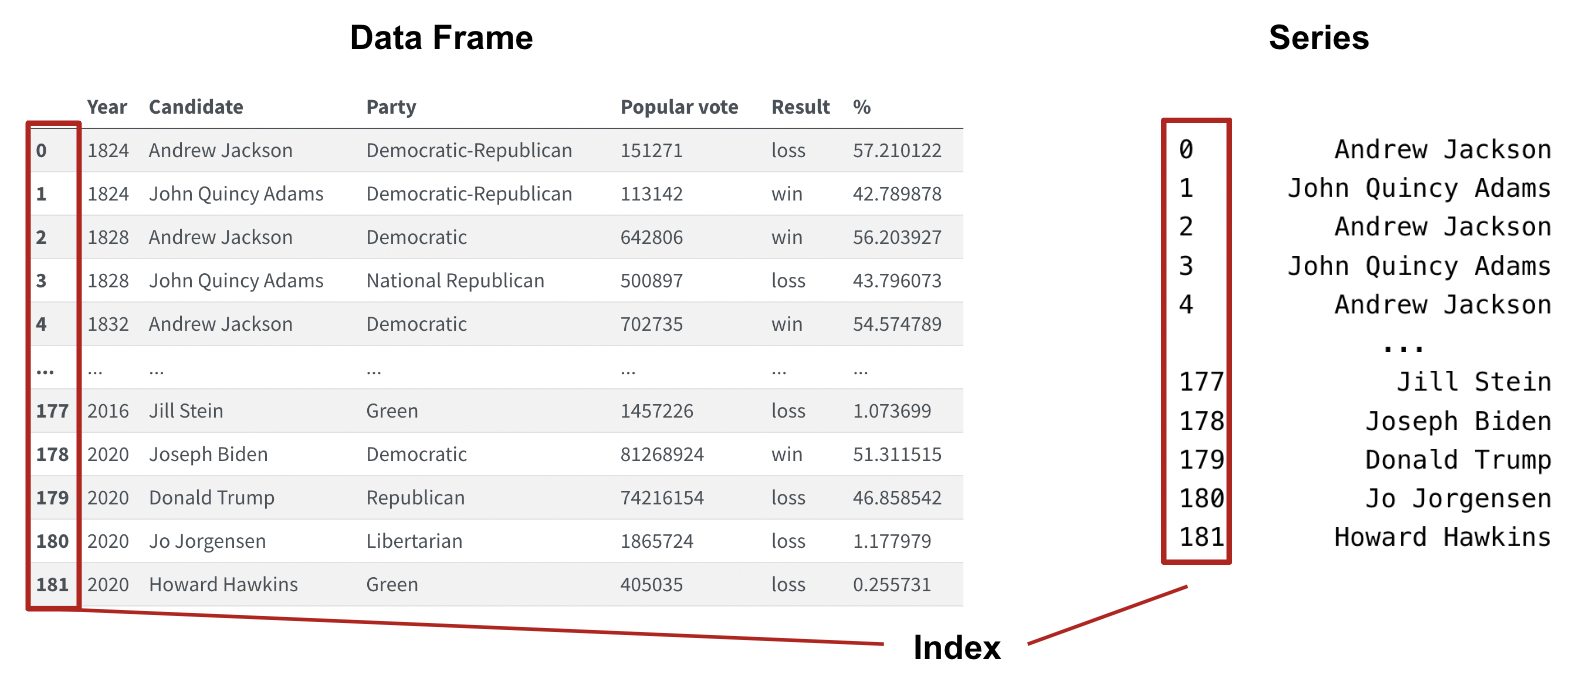
\includegraphics{pandas_1/images/index_comparison_1.png}

However, a DataFrame index doesn't have to be an integer, nor does it
have to be unique. For example, we can set our index to be the name of
our presedential candidates. Selecting a new Series from this modified
DataFrame yields the following:

\begin{Shaded}
\begin{Highlighting}[]
\NormalTok{elections.set\_index(}\StringTok{"Candidate"}\NormalTok{, inplace}\OperatorTok{=}\VariableTok{True}\NormalTok{) }\CommentTok{\# This sets the index to the "Candidate" column}
\end{Highlighting}
\end{Shaded}

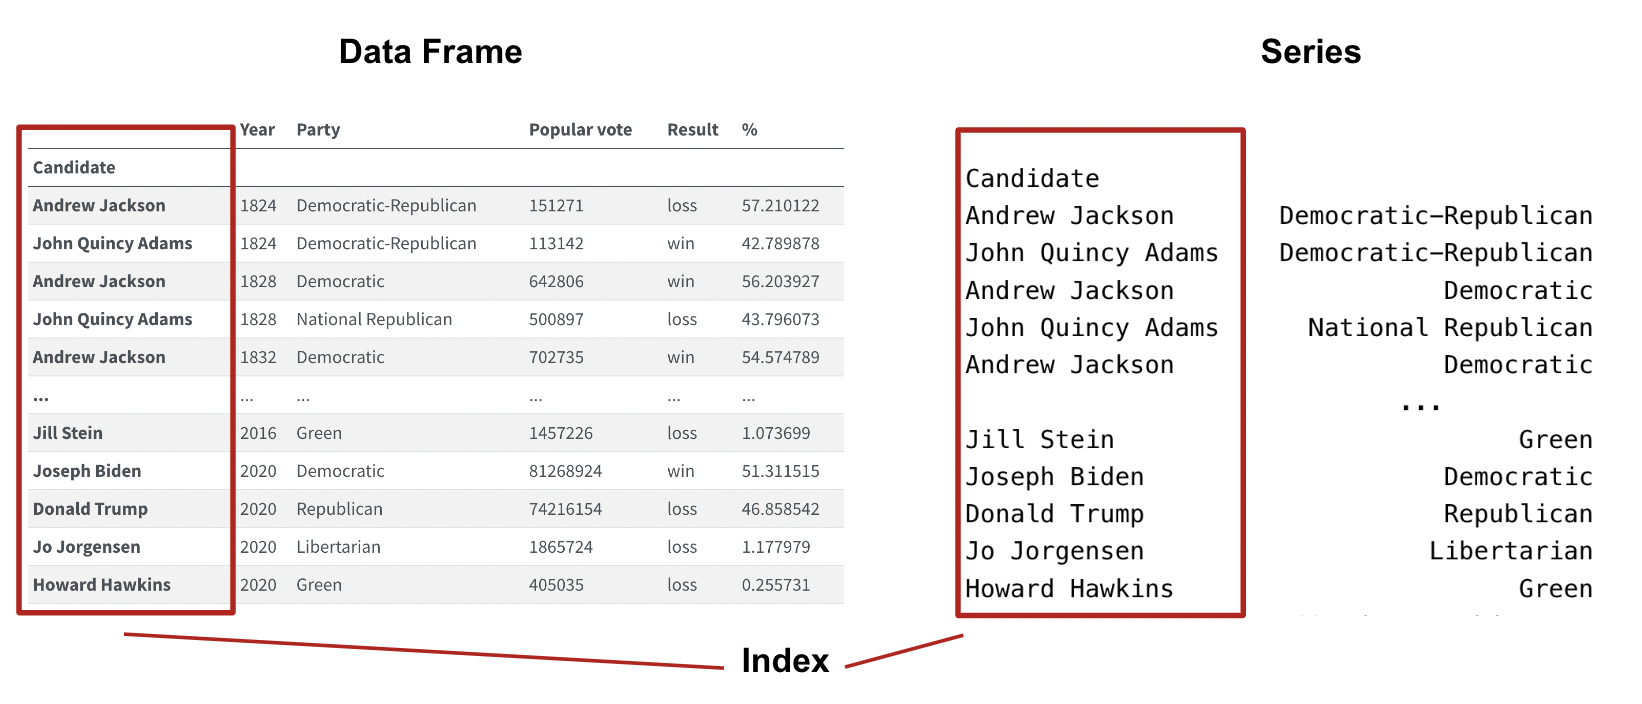
\includegraphics{pandas_1/images/index_comparison_2.png}

To retrieve the indices of a DataFrame, simply use the \texttt{.index}
attribute of the DataFrame class.

\begin{Shaded}
\begin{Highlighting}[]
\NormalTok{elections.index}
\end{Highlighting}
\end{Shaded}

\begin{verbatim}
Index(['Andrew Jackson', 'John Quincy Adams', 'Andrew Jackson',
       'John Quincy Adams', 'Andrew Jackson', 'Henry Clay', 'William Wirt',
       'Hugh Lawson White', 'Martin Van Buren', 'William Henry Harrison',
       ...
       'Darrell Castle', 'Donald Trump', 'Evan McMullin', 'Gary Johnson',
       'Hillary Clinton', 'Jill Stein', 'Joseph Biden', 'Donald Trump',
       'Jo Jorgensen', 'Howard Hawkins'],
      dtype='object', name='Candidate', length=182)
\end{verbatim}

\begin{Shaded}
\begin{Highlighting}[]
\NormalTok{elections.reset\_index(inplace}\OperatorTok{=}\VariableTok{True}\NormalTok{) }\CommentTok{\# This resets the index}
\end{Highlighting}
\end{Shaded}

Earlier, we mentioned that a Series was just a column of data. What if
we wanted a single column as a DataFrame? To obtain this, we can pass in
a list containing a single column to the \texttt{{[}{]}} selection
operator.

\begin{Shaded}
\begin{Highlighting}[]
\NormalTok{elections[[}\StringTok{"Party"}\NormalTok{]] }\CommentTok{\# ["Party"] is the argument {-} a list with a single element}
\end{Highlighting}
\end{Shaded}

\begin{tabular}{ll}
\toprule
{} &                  Party \\
\midrule
0   &  Democratic-Republican \\
1   &  Democratic-Republican \\
2   &             Democratic \\
3   &    National Republican \\
4   &             Democratic \\
5   &    National Republican \\
6   &           Anti-Masonic \\
7   &                   Whig \\
8   &             Democratic \\
9   &                   Whig \\
10  &             Democratic \\
11  &                   Whig \\
12  &                   Whig \\
13  &             Democratic \\
14  &             Democratic \\
15  &              Free Soil \\
16  &                   Whig \\
17  &             Democratic \\
18  &              Free Soil \\
19  &                   Whig \\
20  &             Democratic \\
21  &             Republican \\
22  &               American \\
23  &             Republican \\
24  &   Constitutional Union \\
25  &    Southern Democratic \\
26  &    Northern Democratic \\
27  &         National Union \\
28  &             Democratic \\
29  &             Democratic \\
30  &             Republican \\
31  &     Liberal Republican \\
32  &             Republican \\
33  &             Republican \\
34  &             Democratic \\
35  &              Greenback \\
36  &             Republican \\
37  &             Democratic \\
38  &          Anti-Monopoly \\
39  &             Democratic \\
40  &             Republican \\
41  &            Prohibition \\
42  &            Union Labor \\
43  &             Republican \\
44  &            Prohibition \\
45  &             Democratic \\
46  &             Republican \\
47  &             Democratic \\
48  &               Populist \\
49  &            Prohibition \\
50  &    National Democratic \\
51  &            Prohibition \\
52  &             Democratic \\
53  &             Republican \\
54  &            Prohibition \\
55  &             Democratic \\
56  &             Republican \\
57  &             Democratic \\
58  &              Socialist \\
59  &            Prohibition \\
60  &             Republican \\
61  &               Populist \\
62  &              Socialist \\
63  &            Prohibition \\
64  &             Democratic \\
65  &             Republican \\
66  &              Socialist \\
67  &            Prohibition \\
68  &            Progressive \\
69  &             Republican \\
70  &             Democratic \\
71  &              Socialist \\
72  &             Republican \\
73  &            Prohibition \\
74  &             Democratic \\
75  &            Prohibition \\
76  &              Socialist \\
77  &             Democratic \\
78  &           Farmer–Labor \\
79  &             Republican \\
80  &             Republican \\
81  &             Democratic \\
82  &            Progressive \\
83  &             Democratic \\
84  &             Republican \\
85  &              Socialist \\
86  &             Democratic \\
87  &             Republican \\
88  &              Socialist \\
89  &              Communist \\
90  &             Republican \\
91  &             Democratic \\
92  &              Socialist \\
93  &                  Union \\
94  &             Democratic \\
95  &              Socialist \\
96  &             Republican \\
97  &             Democratic \\
98  &             Republican \\
99  &            Prohibition \\
100 &             Democratic \\
101 &            Progressive \\
102 &              Socialist \\
103 &              Dixiecrat \\
104 &             Republican \\
105 &             Democratic \\
106 &             Republican \\
107 &            Progressive \\
108 &             Democratic \\
109 &             Republican \\
110 &         States' Rights \\
111 &             Democratic \\
112 &             Republican \\
113 &             Republican \\
114 &             Democratic \\
115 &   American Independent \\
116 &             Democratic \\
117 &             Republican \\
118 &             Democratic \\
119 &   American Independent \\
120 &             Republican \\
121 &            Independent \\
122 &             Republican \\
123 &             Democratic \\
124 &   American Independent \\
125 &            Libertarian \\
126 &               American \\
127 &               Citizens \\
128 &            Libertarian \\
129 &             Democratic \\
130 &            Independent \\
131 &             Republican \\
132 &            Libertarian \\
133 &             Republican \\
134 &             Democratic \\
135 &             Republican \\
136 &           New Alliance \\
137 &             Democratic \\
138 &            Libertarian \\
139 &            Libertarian \\
140 &             Democratic \\
141 &               Populist \\
142 &             Republican \\
143 &            Independent \\
144 &             Democratic \\
145 &             Republican \\
146 &            Libertarian \\
147 &              Taxpayers \\
148 &            Natural Law \\
149 &                  Green \\
150 &                 Reform \\
151 &             Democratic \\
152 &             Republican \\
153 &            Libertarian \\
154 &                 Reform \\
155 &                  Green \\
156 &                  Green \\
157 &             Republican \\
158 &             Democratic \\
159 &            Libertarian \\
160 &           Constitution \\
161 &            Independent \\
162 &             Democratic \\
163 &            Libertarian \\
164 &           Constitution \\
165 &                  Green \\
166 &             Republican \\
167 &            Independent \\
168 &             Democratic \\
169 &            Libertarian \\
170 &                  Green \\
171 &             Republican \\
172 &           Constitution \\
173 &             Republican \\
174 &            Independent \\
175 &            Libertarian \\
176 &             Democratic \\
177 &                  Green \\
178 &             Democratic \\
179 &             Republican \\
180 &            Libertarian \\
181 &                  Green \\
\bottomrule
\end{tabular}

\hypertarget{conditional-selection}{%
\section{Conditional Selection}\label{conditional-selection}}

Conditional selection allows us to select a subset of rows in a
DataFrame if they follow some specified condition.

To understand how to use conditional selection, we must look at another
input of the \texttt{.loc} and \texttt{{[}{]}} methods - a boolean
array. This boolean array must have a length equal to the number of rows
in the DataFrame. It will return all rows in the position of a
corresponding \texttt{True} value in the array.

Here, we will select all \emph{even-indexed} rows in the first 10 rows
of our DataFrame.

\begin{Shaded}
\begin{Highlighting}[]
\CommentTok{\# Why is :9 is the correct slice to select the first 10 rows?}
\NormalTok{elections\_first\_10\_rows }\OperatorTok{=}\NormalTok{ elections.loc[:}\DecValTok{9}\NormalTok{, :]}

\CommentTok{\# Notice how we have exactly 10 elements in our boolean array argument}
\NormalTok{elections\_first\_10\_rows[[}\VariableTok{True}\NormalTok{, }\VariableTok{False}\NormalTok{, }\VariableTok{True}\NormalTok{, }\VariableTok{False}\NormalTok{, }\VariableTok{True}\NormalTok{, }\OperatorTok{\textbackslash{}}
                         \VariableTok{False}\NormalTok{, }\VariableTok{True}\NormalTok{, }\VariableTok{False}\NormalTok{, }\VariableTok{True}\NormalTok{, }\VariableTok{False}\NormalTok{]]}
\end{Highlighting}
\end{Shaded}

\begin{tabular}{llrlrlr}
\toprule
{} &         Candidate &  Year &                  Party &  Popular vote & Result &          \% \\
\midrule
0 &    Andrew Jackson &  1824 &  Democratic-Republican &        151271 &   loss &  57.210122 \\
2 &    Andrew Jackson &  1828 &             Democratic &        642806 &    win &  56.203927 \\
4 &    Andrew Jackson &  1832 &             Democratic &        702735 &    win &  54.574789 \\
6 &      William Wirt &  1832 &           Anti-Masonic &        100715 &   loss &   7.821583 \\
8 &  Martin Van Buren &  1836 &             Democratic &        763291 &    win &  52.272472 \\
\bottomrule
\end{tabular}

Unfortunately, using this method to select multiple rows in a large
DataFrame is infeasible. Instead, we can provide a logical condition as
an input to \texttt{.loc} or \texttt{{[}{]}} that returns a boolean
array with said length.

For example, to return all candidates affilliated with the Independent
party:

\begin{Shaded}
\begin{Highlighting}[]
\NormalTok{logical\_operator }\OperatorTok{=}\NormalTok{ elections[}\StringTok{\textquotesingle{}Party\textquotesingle{}}\NormalTok{] }\OperatorTok{==} \StringTok{"Independent"}
\NormalTok{elections[logical\_operator]}
\end{Highlighting}
\end{Shaded}

\begin{tabular}{llrlrlr}
\toprule
{} &         Candidate &  Year &        Party &  Popular vote & Result &          \% \\
\midrule
121 &   Eugene McCarthy &  1976 &  Independent &        740460 &   loss &   0.911649 \\
130 &  John B. Anderson &  1980 &  Independent &       5719850 &   loss &   6.631143 \\
143 &        Ross Perot &  1992 &  Independent &      19743821 &   loss &  18.956298 \\
161 &       Ralph Nader &  2004 &  Independent &        465151 &   loss &   0.380663 \\
167 &       Ralph Nader &  2008 &  Independent &        739034 &   loss &   0.563842 \\
174 &     Evan McMullin &  2016 &  Independent &        732273 &   loss &   0.539546 \\
\bottomrule
\end{tabular}

Here, \texttt{logical\_operator} evaluates to a Series of boolean values
with length 182.

\begin{Shaded}
\begin{Highlighting}[]
\NormalTok{logical\_operator}
\end{Highlighting}
\end{Shaded}

\begin{tabular}{ll}
\toprule
{} &  Party \\
\midrule
0   &  False \\
1   &  False \\
2   &  False \\
3   &  False \\
4   &  False \\
5   &  False \\
6   &  False \\
7   &  False \\
8   &  False \\
9   &  False \\
10  &  False \\
11  &  False \\
12  &  False \\
13  &  False \\
14  &  False \\
15  &  False \\
16  &  False \\
17  &  False \\
18  &  False \\
19  &  False \\
20  &  False \\
21  &  False \\
22  &  False \\
23  &  False \\
24  &  False \\
25  &  False \\
26  &  False \\
27  &  False \\
28  &  False \\
29  &  False \\
30  &  False \\
31  &  False \\
32  &  False \\
33  &  False \\
34  &  False \\
35  &  False \\
36  &  False \\
37  &  False \\
38  &  False \\
39  &  False \\
40  &  False \\
41  &  False \\
42  &  False \\
43  &  False \\
44  &  False \\
45  &  False \\
46  &  False \\
47  &  False \\
48  &  False \\
49  &  False \\
50  &  False \\
51  &  False \\
52  &  False \\
53  &  False \\
54  &  False \\
55  &  False \\
56  &  False \\
57  &  False \\
58  &  False \\
59  &  False \\
60  &  False \\
61  &  False \\
62  &  False \\
63  &  False \\
64  &  False \\
65  &  False \\
66  &  False \\
67  &  False \\
68  &  False \\
69  &  False \\
70  &  False \\
71  &  False \\
72  &  False \\
73  &  False \\
74  &  False \\
75  &  False \\
76  &  False \\
77  &  False \\
78  &  False \\
79  &  False \\
80  &  False \\
81  &  False \\
82  &  False \\
83  &  False \\
84  &  False \\
85  &  False \\
86  &  False \\
87  &  False \\
88  &  False \\
89  &  False \\
90  &  False \\
91  &  False \\
92  &  False \\
93  &  False \\
94  &  False \\
95  &  False \\
96  &  False \\
97  &  False \\
98  &  False \\
99  &  False \\
100 &  False \\
101 &  False \\
102 &  False \\
103 &  False \\
104 &  False \\
105 &  False \\
106 &  False \\
107 &  False \\
108 &  False \\
109 &  False \\
110 &  False \\
111 &  False \\
112 &  False \\
113 &  False \\
114 &  False \\
115 &  False \\
116 &  False \\
117 &  False \\
118 &  False \\
119 &  False \\
120 &  False \\
121 &   True \\
122 &  False \\
123 &  False \\
124 &  False \\
125 &  False \\
126 &  False \\
127 &  False \\
128 &  False \\
129 &  False \\
130 &   True \\
131 &  False \\
132 &  False \\
133 &  False \\
134 &  False \\
135 &  False \\
136 &  False \\
137 &  False \\
138 &  False \\
139 &  False \\
140 &  False \\
141 &  False \\
142 &  False \\
143 &   True \\
144 &  False \\
145 &  False \\
146 &  False \\
147 &  False \\
148 &  False \\
149 &  False \\
150 &  False \\
151 &  False \\
152 &  False \\
153 &  False \\
154 &  False \\
155 &  False \\
156 &  False \\
157 &  False \\
158 &  False \\
159 &  False \\
160 &  False \\
161 &   True \\
162 &  False \\
163 &  False \\
164 &  False \\
165 &  False \\
166 &  False \\
167 &   True \\
168 &  False \\
169 &  False \\
170 &  False \\
171 &  False \\
172 &  False \\
173 &  False \\
174 &   True \\
175 &  False \\
176 &  False \\
177 &  False \\
178 &  False \\
179 &  False \\
180 &  False \\
181 &  False \\
\bottomrule
\end{tabular}

Rows 121, 130, 143, 161, 167, and 174 evaluate to \texttt{True} and are
thus returned in the DataFrame.

\begin{Shaded}
\begin{Highlighting}[]
\BuiltInTok{print}\NormalTok{(logical\_operator.loc[[}\DecValTok{121}\NormalTok{, }\DecValTok{130}\NormalTok{, }\DecValTok{143}\NormalTok{, }\DecValTok{161}\NormalTok{, }\DecValTok{167}\NormalTok{, }\DecValTok{174}\NormalTok{]])}
\end{Highlighting}
\end{Shaded}

\begin{verbatim}
121    True
130    True
143    True
161    True
167    True
174    True
Name: Party, dtype: bool
\end{verbatim}

Passing a Series as an argument to \texttt{elections{[}{]}} has the same
affect as using a boolean array. In fact, the \texttt{{[}{]}} selection
operator can take a boolean Series, array, and list as arguments. These
three are used interchangeably thoughout the course.

Similarly, we can use \texttt{.loc} to achieve similar results.

\begin{Shaded}
\begin{Highlighting}[]
\NormalTok{elections.loc[elections[}\StringTok{\textquotesingle{}Party\textquotesingle{}}\NormalTok{] }\OperatorTok{==} \StringTok{"Independent"}\NormalTok{]}
\end{Highlighting}
\end{Shaded}

\begin{tabular}{llrlrlr}
\toprule
{} &         Candidate &  Year &        Party &  Popular vote & Result &          \% \\
\midrule
121 &   Eugene McCarthy &  1976 &  Independent &        740460 &   loss &   0.911649 \\
130 &  John B. Anderson &  1980 &  Independent &       5719850 &   loss &   6.631143 \\
143 &        Ross Perot &  1992 &  Independent &      19743821 &   loss &  18.956298 \\
161 &       Ralph Nader &  2004 &  Independent &        465151 &   loss &   0.380663 \\
167 &       Ralph Nader &  2008 &  Independent &        739034 &   loss &   0.563842 \\
174 &     Evan McMullin &  2016 &  Independent &        732273 &   loss &   0.539546 \\
\bottomrule
\end{tabular}

Boolean conditions can be combined using various operators that allow us
to filter results by multiple conditions. Some examples include the
\texttt{\&} (and) operator and \texttt{\textbar{}} (or) operator.

\textbf{Note}: When combining multiple conditions with logical
operators, be sure to surround each condition with a set of paranthesis
\texttt{()}. If you forget, your code will throw an error.

For example, if we want to return data on all presidential candidates
affiliated with the Independent Party before the 21\textsuperscript{st}
century, we can do so:

\begin{Shaded}
\begin{Highlighting}[]
\NormalTok{elections[(elections[}\StringTok{\textquotesingle{}Party\textquotesingle{}}\NormalTok{] }\OperatorTok{==} \StringTok{"Independent"}\NormalTok{) }\OperatorTok{\textbackslash{}}
          \OperatorTok{\&}\NormalTok{ (elections[}\StringTok{\textquotesingle{}Year\textquotesingle{}}\NormalTok{] }\OperatorTok{\textless{}} \DecValTok{2000}\NormalTok{)]}
\end{Highlighting}
\end{Shaded}

\begin{tabular}{llrlrlr}
\toprule
{} &         Candidate &  Year &        Party &  Popular vote & Result &          \% \\
\midrule
121 &   Eugene McCarthy &  1976 &  Independent &        740460 &   loss &   0.911649 \\
130 &  John B. Anderson &  1980 &  Independent &       5719850 &   loss &   6.631143 \\
143 &        Ross Perot &  1992 &  Independent &      19743821 &   loss &  18.956298 \\
\bottomrule
\end{tabular}

\hypertarget{handy-utility-functions}{%
\section{Handy Utility Functions}\label{handy-utility-functions}}

There are a large number of operations supported by \texttt{pandas} that
allow us to efficiently manipulate data. In this section, we'll cover a
few.

\begin{enumerate}
\def\labelenumi{\arabic{enumi}.}
\tightlist
\item
  \texttt{.head} and \texttt{.tail}
\item
  \texttt{.shape} and \texttt{.size}
\item
  \texttt{.describe}
\item
  \texttt{.sample}
\item
  \texttt{.value\_counts}
\item
  \texttt{.unique}
\item
  \texttt{.sort\_values}
\end{enumerate}

\hypertarget{head-.tail}{%
\subsubsection{.head / .tail}\label{head-.tail}}

\texttt{.head(n)} and \texttt{.tail(n)} display the first \texttt{n} and
last \texttt{n} rows of a DataFrame, respectively.

\begin{Shaded}
\begin{Highlighting}[]
\NormalTok{elections.head(}\DecValTok{3}\NormalTok{)}
\end{Highlighting}
\end{Shaded}

\begin{tabular}{llrlrlr}
\toprule
{} &          Candidate &  Year &                  Party &  Popular vote & Result &          \% \\
\midrule
0 &     Andrew Jackson &  1824 &  Democratic-Republican &        151271 &   loss &  57.210122 \\
1 &  John Quincy Adams &  1824 &  Democratic-Republican &        113142 &    win &  42.789878 \\
2 &     Andrew Jackson &  1828 &             Democratic &        642806 &    win &  56.203927 \\
\bottomrule
\end{tabular}

\begin{Shaded}
\begin{Highlighting}[]
\NormalTok{elections.tail(}\DecValTok{3}\NormalTok{)}
\end{Highlighting}
\end{Shaded}

\begin{tabular}{llrlrlr}
\toprule
{} &       Candidate &  Year &        Party &  Popular vote & Result &          \% \\
\midrule
179 &    Donald Trump &  2020 &   Republican &      74216154 &   loss &  46.858542 \\
180 &    Jo Jorgensen &  2020 &  Libertarian &       1865724 &   loss &   1.177979 \\
181 &  Howard Hawkins &  2020 &        Green &        405035 &   loss &   0.255731 \\
\bottomrule
\end{tabular}

\hypertarget{shape-.size}{%
\subsubsection{.shape / .size}\label{shape-.size}}

\texttt{.shape} returns a tuple with the number of rows and columns in a
DataFrame. \texttt{.size} returns the total number of data entries. This
is the product of the number of rows and columns.

\begin{Shaded}
\begin{Highlighting}[]
\NormalTok{elections.shape}
\end{Highlighting}
\end{Shaded}

\begin{verbatim}
(182, 6)
\end{verbatim}

\begin{Shaded}
\begin{Highlighting}[]
\NormalTok{num\_rows, num\_cols }\OperatorTok{=}\NormalTok{ elections.shape}
\ControlFlowTok{assert}\NormalTok{(elections.size }\OperatorTok{==}\NormalTok{ num\_rows }\OperatorTok{*}\NormalTok{ num\_cols)}
\NormalTok{elections.size}
\end{Highlighting}
\end{Shaded}

\begin{verbatim}
1092
\end{verbatim}

\hypertarget{describe}{%
\subsubsection{.describe}\label{describe}}

\texttt{.describe()} returns a DataFrame of useful summary statistics
for each numerical column.

\begin{Shaded}
\begin{Highlighting}[]
\NormalTok{elections.describe()}
\end{Highlighting}
\end{Shaded}

\begin{tabular}{lrrr}
\toprule
{} &         Year &  Popular vote &           \% \\
\midrule
count &   182.000000 &  1.820000e+02 &  182.000000 \\
mean  &  1934.087912 &  1.235364e+07 &   27.470350 \\
std   &    57.048908 &  1.907715e+07 &   22.968034 \\
min   &  1824.000000 &  1.007150e+05 &    0.098088 \\
25\%   &  1889.000000 &  3.876395e+05 &    1.219996 \\
50\%   &  1936.000000 &  1.709375e+06 &   37.677893 \\
75\%   &  1988.000000 &  1.897775e+07 &   48.354977 \\
max   &  2020.000000 &  8.126892e+07 &   61.344703 \\
\bottomrule
\end{tabular}

\hypertarget{sample}{%
\subsubsection{.sample}\label{sample}}

\texttt{.sample(n)} returns a random sample of \texttt{n} rows from the
given DataFrame.

\begin{Shaded}
\begin{Highlighting}[]
\NormalTok{elections.sample(}\DecValTok{3}\NormalTok{)}
\end{Highlighting}
\end{Shaded}

\begin{tabular}{llrlrlr}
\toprule
{} &         Candidate &  Year &        Party &  Popular vote & Result &          \% \\
\midrule
75 &  Aaron S. Watkins &  1920 &  Prohibition &        188787 &   loss &   0.708351 \\
95 &     Norman Thomas &  1940 &    Socialist &        116599 &   loss &   0.234237 \\
22 &  Millard Fillmore &  1856 &     American &        873053 &   loss &  21.554001 \\
\bottomrule
\end{tabular}

\hypertarget{value_counts}{%
\subsubsection{.value\_counts}\label{value_counts}}

\texttt{.value\_counts()} is called on a column and returns a Series
containing the total count of each unique value.

\begin{Shaded}
\begin{Highlighting}[]
\NormalTok{elections[}\StringTok{\textquotesingle{}Candidate\textquotesingle{}}\NormalTok{].value\_counts()}
\end{Highlighting}
\end{Shaded}

\begin{tabular}{lr}
\toprule
{} &  Candidate \\
\midrule
Norman Thomas          &          5 \\
Ralph Nader            &          4 \\
Eugene V. Debs         &          4 \\
Franklin Roosevelt     &          4 \\
Andrew Jackson         &          3 \\
William Jennings Bryan &          3 \\
Martin Van Buren       &          3 \\
Grover Cleveland       &          3 \\
Richard Nixon          &          3 \\
Barack Obama           &          2 \\
Jill Stein             &          2 \\
Eugene W. Chafin       &          2 \\
Henry Clay             &          2 \\
Jimmy Carter           &          2 \\
Ronald Reagan          &          2 \\
William Taft           &          2 \\
James B. Weaver        &          2 \\
Herbert Hoover         &          2 \\
Bill Clinton           &          2 \\
Theodore Roosevelt     &          2 \\
Woodrow Wilson         &          2 \\
John Quincy Adams      &          2 \\
Ross Perot             &          2 \\
Benjamin Harrison      &          2 \\
Thomas E. Dewey        &          2 \\
George W. Bush         &          2 \\
Dwight Eisenhower      &          2 \\
Donald Trump           &          2 \\
Gary Johnson           &          2 \\
William Henry Harrison &          2 \\
Harry Browne           &          2 \\
Abraham Lincoln        &          2 \\
Adlai Stevenson        &          2 \\
William McKinley       &          2 \\
Ulysses Grant          &          2 \\
George H. W. Bush      &          2 \\
Lenora Fulani          &          1 \\
Al Gore                &          1 \\
Hillary Clinton        &          1 \\
James Garfield         &          1 \\
Calvin Coolidge        &          1 \\
Howard Phillips        &          1 \\
Ed Clark               &          1 \\
James Polk             &          1 \\
Bo Gritz               &          1 \\
Harry Truman           &          1 \\
Aaron S. Watkins       &          1 \\
Vincent Hallinan       &          1 \\
Frank Hanly            &          1 \\
David Bergland         &          1 \\
Claude A. Watson       &          1 \\
Horace Greeley         &          1 \\
Gerald Ford            &          1 \\
Warren Harding         &          1 \\
Parley P. Christensen  &          1 \\
Barry Commoner         &          1 \\
David Cobb             &          1 \\
George B. McClellan    &          1 \\
Michael Peroutka       &          1 \\
John Hagelin           &          1 \\
William Wirt           &          1 \\
Joshua Levering        &          1 \\
John W. Davis          &          1 \\
Silas C. Swallow       &          1 \\
George McGovern        &          1 \\
Millard Fillmore       &          1 \\
Eugene McCarthy        &          1 \\
Evan McMullin          &          1 \\
John Kerry             &          1 \\
Lester Maddox          &          1 \\
Thomas J. Anderson     &          1 \\
Lewis Cass             &          1 \\
John Bidwell           &          1 \\
Stephen A. Douglas     &          1 \\
Roger MacBride         &          1 \\
John G. Schmitz        &          1 \\
Robert La Follette     &          1 \\
Joseph Biden           &          1 \\
Franklin Pierce        &          1 \\
John C. Frémont        &          1 \\
Alson Streeter         &          1 \\
Cynthia McKinney       &          1 \\
Allan L. Benson        &          1 \\
Alf Landon             &          1 \\
John St. John          &          1 \\
Jo Jorgensen           &          1 \\
James M. Cox           &          1 \\
T. Coleman Andrews     &          1 \\
Horatio Seymour        &          1 \\
Chuck Baldwin          &          1 \\
John B. Anderson       &          1 \\
Clinton B. Fisk        &          1 \\
Mitt Romney            &          1 \\
Rutherford Hayes       &          1 \\
John McCain            &          1 \\
Benjamin Butler        &          1 \\
Pat Buchanan           &          1 \\
Lyndon Johnson         &          1 \\
Zachary Taylor         &          1 \\
William Z. Foster      &          1 \\
Henry A. Wallace       &          1 \\
Bob Dole               &          1 \\
Andre Marrou           &          1 \\
James Buchanan         &          1 \\
Howard Hawkins         &          1 \\
John Bell              &          1 \\
Ron Paul               &          1 \\
Hugh Lawson White      &          1 \\
Barry Goldwater        &          1 \\
James G. Blaine        &          1 \\
John Kennedy           &          1 \\
John M. Palmer         &          1 \\
John C. Breckinridge   &          1 \\
Al Smith               &          1 \\
Hubert Humphrey        &          1 \\
Walter Mondale         &          1 \\
Michael Badnarik       &          1 \\
Charles Evans Hughes   &          1 \\
George Wallace         &          1 \\
Samuel J. Tilden       &          1 \\
Winfield Scott Hancock &          1 \\
Wendell Willkie        &          1 \\
Winfield Scott         &          1 \\
Michael Dukakis        &          1 \\
John P. Hale           &          1 \\
Alton B. Parker        &          1 \\
Darrell Castle         &          1 \\
William Lemke          &          1 \\
Strom Thurmond         &          1 \\
Bob Barr               &          1 \\
John G. Woolley        &          1 \\
Thomas E. Watson       &          1 \\
\bottomrule
\end{tabular}

This code tells us how many times each candidate ran for president of
the United States.

\hypertarget{unique}{%
\subsubsection{.unique}\label{unique}}

\texttt{.unique()} is called on a Series and returns an array with its
unique values.

\begin{Shaded}
\begin{Highlighting}[]
\CommentTok{\# For brevity, we have limited the results to 5 candidates }
\NormalTok{elections[}\StringTok{\textquotesingle{}Candidate\textquotesingle{}}\NormalTok{].unique()[:}\DecValTok{5}\NormalTok{]}
\end{Highlighting}
\end{Shaded}

\begin{verbatim}
array(['Andrew Jackson', 'John Quincy Adams', 'Henry Clay',
       'William Wirt', 'Hugh Lawson White'], dtype=object)
\end{verbatim}

\hypertarget{sort_values}{%
\subsubsection{.sort\_values}\label{sort_values}}

\texttt{.sort\_values()} returns a sorted version of the Series it was
called on. Numerical values are in sorted magnitude, while text is
sorted in alphabetical order. You may specify optional arguments to sort
in ascending or descending order.

\begin{Shaded}
\begin{Highlighting}[]
\NormalTok{elections[}\StringTok{\textquotesingle{}Candidate\textquotesingle{}}\NormalTok{].sort\_values()}
\end{Highlighting}
\end{Shaded}

\begin{tabular}{ll}
\toprule
{} &               Candidate \\
\midrule
75  &        Aaron S. Watkins \\
27  &         Abraham Lincoln \\
23  &         Abraham Lincoln \\
108 &         Adlai Stevenson \\
105 &         Adlai Stevenson \\
151 &                 Al Gore \\
83  &                Al Smith \\
90  &              Alf Landon \\
71  &         Allan L. Benson \\
42  &          Alson Streeter \\
57  &         Alton B. Parker \\
139 &            Andre Marrou \\
0   &          Andrew Jackson \\
2   &          Andrew Jackson \\
4   &          Andrew Jackson \\
162 &            Barack Obama \\
168 &            Barack Obama \\
127 &          Barry Commoner \\
113 &         Barry Goldwater \\
38  &         Benjamin Butler \\
43  &       Benjamin Harrison \\
46  &       Benjamin Harrison \\
140 &            Bill Clinton \\
144 &            Bill Clinton \\
141 &                Bo Gritz \\
163 &                Bob Barr \\
145 &                Bob Dole \\
80  &         Calvin Coolidge \\
72  &    Charles Evans Hughes \\
164 &           Chuck Baldwin \\
99  &        Claude A. Watson \\
44  &         Clinton B. Fisk \\
165 &        Cynthia McKinney \\
172 &          Darrell Castle \\
132 &          David Bergland \\
156 &              David Cobb \\
179 &            Donald Trump \\
173 &            Donald Trump \\
109 &       Dwight Eisenhower \\
106 &       Dwight Eisenhower \\
128 &                Ed Clark \\
121 &         Eugene McCarthy \\
66  &          Eugene V. Debs \\
62  &          Eugene V. Debs \\
58  &          Eugene V. Debs \\
76  &          Eugene V. Debs \\
67  &        Eugene W. Chafin \\
63  &        Eugene W. Chafin \\
174 &           Evan McMullin \\
73  &             Frank Hanly \\
17  &         Franklin Pierce \\
91  &      Franklin Roosevelt \\
94  &      Franklin Roosevelt \\
86  &      Franklin Roosevelt \\
97  &      Franklin Roosevelt \\
175 &            Gary Johnson \\
169 &            Gary Johnson \\
28  &     George B. McClellan \\
135 &       George H. W. Bush \\
142 &       George H. W. Bush \\
118 &         George McGovern \\
157 &          George W. Bush \\
152 &          George W. Bush \\
115 &          George Wallace \\
122 &             Gerald Ford \\
45  &        Grover Cleveland \\
39  &        Grover Cleveland \\
47  &        Grover Cleveland \\
146 &            Harry Browne \\
153 &            Harry Browne \\
100 &            Harry Truman \\
101 &        Henry A. Wallace \\
12  &              Henry Clay \\
5   &              Henry Clay \\
87  &          Herbert Hoover \\
84  &          Herbert Hoover \\
176 &         Hillary Clinton \\
31  &          Horace Greeley \\
29  &         Horatio Seymour \\
181 &          Howard Hawkins \\
147 &         Howard Phillips \\
116 &         Hubert Humphrey \\
7   &       Hugh Lawson White \\
35  &         James B. Weaver \\
48  &         James B. Weaver \\
20  &          James Buchanan \\
40  &         James G. Blaine \\
36  &          James Garfield \\
77  &            James M. Cox \\
13  &              James Polk \\
177 &              Jill Stein \\
170 &              Jill Stein \\
129 &            Jimmy Carter \\
123 &            Jimmy Carter \\
180 &            Jo Jorgensen \\
130 &        John B. Anderson \\
24  &               John Bell \\
49  &            John Bidwell \\
25  &    John C. Breckinridge \\
21  &         John C. Frémont \\
119 &         John G. Schmitz \\
54  &         John G. Woolley \\
148 &            John Hagelin \\
111 &            John Kennedy \\
158 &              John Kerry \\
50  &          John M. Palmer \\
166 &             John McCain \\
18  &            John P. Hale \\
1   &       John Quincy Adams \\
3   &       John Quincy Adams \\
41  &           John St. John \\
81  &           John W. Davis \\
178 &            Joseph Biden \\
51  &         Joshua Levering \\
136 &           Lenora Fulani \\
124 &           Lester Maddox \\
14  &              Lewis Cass \\
114 &          Lyndon Johnson \\
15  &        Martin Van Buren \\
8   &        Martin Van Buren \\
10  &        Martin Van Buren \\
159 &        Michael Badnarik \\
137 &         Michael Dukakis \\
160 &        Michael Peroutka \\
22  &        Millard Fillmore \\
171 &             Mitt Romney \\
85  &           Norman Thomas \\
95  &           Norman Thomas \\
92  &           Norman Thomas \\
88  &           Norman Thomas \\
102 &           Norman Thomas \\
78  &   Parley P. Christensen \\
154 &            Pat Buchanan \\
155 &             Ralph Nader \\
149 &             Ralph Nader \\
161 &             Ralph Nader \\
167 &             Ralph Nader \\
120 &           Richard Nixon \\
117 &           Richard Nixon \\
112 &           Richard Nixon \\
82  &      Robert La Follette \\
125 &          Roger MacBride \\
138 &                Ron Paul \\
131 &           Ronald Reagan \\
133 &           Ronald Reagan \\
143 &              Ross Perot \\
150 &              Ross Perot \\
33  &        Rutherford Hayes \\
34  &        Samuel J. Tilden \\
59  &        Silas C. Swallow \\
26  &      Stephen A. Douglas \\
103 &          Strom Thurmond \\
110 &      T. Coleman Andrews \\
68  &      Theodore Roosevelt \\
60  &      Theodore Roosevelt \\
98  &         Thomas E. Dewey \\
104 &         Thomas E. Dewey \\
61  &        Thomas E. Watson \\
126 &      Thomas J. Anderson \\
32  &           Ulysses Grant \\
30  &           Ulysses Grant \\
107 &        Vincent Hallinan \\
134 &          Walter Mondale \\
79  &          Warren Harding \\
96  &         Wendell Willkie \\
11  &  William Henry Harrison \\
9   &  William Henry Harrison \\
55  &  William Jennings Bryan \\
52  &  William Jennings Bryan \\
64  &  William Jennings Bryan \\
93  &           William Lemke \\
53  &        William McKinley \\
56  &        William McKinley \\
69  &            William Taft \\
65  &            William Taft \\
6   &            William Wirt \\
89  &       William Z. Foster \\
19  &          Winfield Scott \\
37  &  Winfield Scott Hancock \\
74  &          Woodrow Wilson \\
70  &          Woodrow Wilson \\
16  &          Zachary Taylor \\
\bottomrule
\end{tabular}

\hypertarget{parting-note}{%
\subsection{Parting Note}\label{parting-note}}

The \texttt{pandas} library is enormous and contains many useful
functions. Here is a link to
\href{https://pandas.pydata.org/docs/}{documentation}.

This lecture and the next will cover important methods you should be
fluent in. However, we want you to get familiar with the real world
programming practice of \ldots Googling! Answers to your questions can
be found in documentation, Stack Overflow, etc.

With that, let's move on to Pandas II.



\end{document}
